\documentclass[a4paper,12pt]{report} %размер бумаги устанавливаем А4, шрифт 14пунктов
\usepackage[T2A]{fontenc}
\usepackage[utf8]{inputenc}%включаем свою кодировку: koi8-r или utf8 в UNIX, cp1251 в Windows
\usepackage[english,russian]{babel}%используем русский и английский языки с переносами
\usepackage{amssymb,amsfonts,amsmath,cite,enumerate,float,caption} %подключаем нужные пакеты расширений
\usepackage[pdftex]{graphicx} %хотим вставлять в диплом рисунки?
\graphicspath{{images/}{images/Meas POR_NOR/}}%путь к рисункам}
\usepackage[labelsep=period]{caption} %точка в подписях
\usepackage[
  locale = DE % comma as decimal mark
]{siunitx}
\makeatletter
\renewcommand{\@biblabel}[1]{#1.} % Заменяем библиографию с квадратных скобок на точку:
\makeatother

\usepackage{multirow} %объединение строк таблиц
\usepackage{multicol} %объединение столбцов таблиц
\usepackage{color} %цвет таблиц
\usepackage{colortbl} %цвет таблиц
\usepackage{bigstrut} %для таблиц
\usepackage{rotating}


\usepackage[strict]{changepage} %для смены границ полей

\usepackage{geometry} % Меняем поля страницы
\geometry{left=2cm}% левое поле
\geometry{right=1.5cm}% правое поле
\geometry{top=1cm}% верхнее поле
\geometry{bottom=2cm}% нижнее поле

\setlength{\parindent}{1cm} % настройка красной строки

\captionsetup[table]{singlelinecheck=false,justification=raggedleft} %выравнивание по правому краю заголовков таблиц

\renewcommand{\theenumi}{\arabic{enumi}}% Меняем везде перечисления на цифра.цифра
\renewcommand{\labelenumi}{\arabic{enumi}}% Меняем везде перечисления на цифра.цифра
\renewcommand{\theenumii}{.\arabic{enumii}}% Меняем везде перечисления на цифра.цифра
\renewcommand{\labelenumii}{\arabic{enumi}.\arabic{enumii}.}% Меняем везде перечисления на цифра.цифра
\renewcommand{\theenumiii}{.\arabic{enumiii}}% Меняем везде перечисления на цифра.цифра
\renewcommand{\labelenumiii}{\arabic{enumi}.\arabic{enumii}.\arabic{enumiii}.}% Меняем везде перечисления на цифра.цифра
\renewcommand{\thefigure}{\thesection.\arabic{figure}} % меням вид нумерации рисунков 
\renewcommand{\thetable}{\thesection.\arabic{table}} % меням вид нумерации таблиц
\renewcommand{\labelenumi}{\arabic{enumi}.} % меняем вид нумерованных списков
%\renewcommand{\equation}{\arabic{enumi}.} % меняем вид нумерации формул

\begin{document}
\begin{titlepage}
    \newpage
    
    \begin{center}
    ПРАВИТЕЛЬСТВО РОССИЙСКОЙ ФЕДЕРАЦИИ \\
    \vspace{1em}
    ФЕДЕРАЛЬНОЕ  ГОСУДАРСТВЕННОЕ АВТОНОМНОЕ \\
    ОБРАЗОВАТЕЛЬНОЕ УЧРЕЖДЕНИЕ ВЫСШЕГО ОБРАЗОВАНИЯ \\
    <<НАЦИОНАЛЬНЫЙ ИССЛЕДОВАТЕЛЬСКИЙ УНИВЕРСИТЕТ \\
    <<ВЫСШАЯ ШКОЛА ЭКОНОМИК>> \\
    \vspace{2em}
    \textbf{Московский институт электроники и математики им. А.Н. Тихонова}\\
    \vspace{6em}
    Степушин Кирилл Алексеевич\\
    \vspace{3em}
    \textbf{РАЗРАБОТКА ОТЛАДЧИКА С МОНИТОРИНГОМ ЭНЕРГОПОТРЕБЛЕНИЯ}\\
    \vspace{6em}
    Выпускная квалификационная работа -- магистерская диссертация\\ 
    по направлению 11.04.02 «Инфокоммуникационные технологии и системы связи»\\
    студента образовательной программы магистратуры\\
    «Интернет вещей и киберфизические системы»
    \end{center}

    \vspace{6em}

    \begin{flushleft}
    Студент \hfill Научный руководитель\\
    \hfill приглашенный преподаватель\\
    \vspace{1em}
    \rule{5cm}{0.005cm} \hfill \rule{5cm}{0.01cm}\\
    \hfill И.О.Фамилия

    \vspace{1em}

    Рецензент \hfill Консультант\\
    к.т.н., доцент \hfill приглашенный преподаватель\\
    \vspace{1em}
    \rule{5cm}{0.005cm} \hfill \rule{5cm}{0.01cm}\\
    И.О.Фамилия \hfill И.О.Фамилия
    \end{flushleft}
    
    \vspace{\fill}
    
    \begin{center}
    Москва 2024
    \end{center}
    
    \end{titlepage}%титульный лист
\tableofcontents %оглавление, которое генерируется автоматически

\chapter*{Введение}
\addcontentsline{toc}{chapter}{Введение}
\hspace{1cm} Независимо от стараний разработчика или сложности проекта, большая часть времени разработки
будет потрачена на то, чтобы убедиться, что устройство работает правильно, или -- что наиболее
вероятно -- разобраться, почему устройство работает не так, как ожидалось. Отладчик -- самый мощный 
инструмент в наборе инструментов разработчика, позволяющий напрямую взаимодействовать с процессором,
задавать точки останова, пошагово управлять потоком выполнения инструкций и проверять  значения
регистров. \cite{Lakamera:embed}

Для устройств <<интернета вещей>> очень важно знать и отслеживать энергопотребление,
ведь обычно такие устройства питаются от батарейки и каждое ненужное действие уменьшит
срок службы. Мониторинг энергопотребления позволяет понять энергоэффективность каждого сеанса связи,
что позволит выбрать наиболее подходящий интерфейс и протокол передачи данных.

Об актуальности возможности мониторинга энергопотребления для отладчика говорит количество 
измерительных устройств на рынке. Характеристики основных из них приведены в таблице 
\ref{comparemeasdevices}.

\begin{table}[H]
    \caption{Сравнение характеристик измерительных устройств}
    \label{comparemeasdevices}   
    \begin{center}
    \begin{tabular}{|c|c|c|c|c|}
    \hline
  Устройство & Joulescope & Otii Arc & NanoRanger & Current Ranger \\ \hline
    Диапазон тока & от -1 А до 3 А & от 0 до 2,5 А & от 1 нА до 800 мА & от -1,65 А до 3 А \\ \hline
    Разрешение & 1 нА & десятки нА & до 10 пА & до 1 пА  \\ \hline
    Погрешность & до 0,3\% & до 0,1\% & до 0,3\% & до 0,1\% \\ \hline
    Цена & 800 \$ & 700 \$ & 220 \$ & 120 \$  \\ \hline
    \end{tabular}
    \end{center}
\end{table} 

Так же о высокой потребности в устройстве говорит большое количество существующих отладчиков с 
мониторингом энергопотребления от различных производителей микроконтроллеров, например STLINK-V3 
\cite{STLINKV3} и Power Profiler Kit II \cite{Power Profiler Kit}, так и от сторонних компаний, например 
Energymon.

Потребность в таком отладчике также имеется у MIEM IoT-LAB для реализации возможности удаленного 
мониторинга энергопотребления, как как это сделано в оригинале у FIT IoT-LAB, а так же улучшение 
французского решения в сторону замены аппаратной реализации с PaspBerry на микроконтроллер и повышения 
точности и качества мониторинга потребляемой мощности у отлаживаемых устройств. \cite{FITIoT}.

Определяя требования к диапазонам измеряемого тока, стоит учитывать различные IoT-устройства. Грубую оценку
можно составить на примере Wi-Fi решений и сотовых модемов, которые в <<пике>> передачи данных могут 
иметь потребление в районе одного ампера, а в спящем режиме потребляют порядка единиц мкА.

%ссылку на инфу

Перед проектированием отладчика с возможностью мониторинга энергопотребления IoT-устройств
следует определиться с требованиями, предъявляемыми к отладчику. 
Для этого в качестве примера рассмотрим <<усредненный>> паттерн поведения устройства с BLE, одной
из самых популярных технологий беспроводной передачи данных интернета вещей, 
у которого с периодичностью в несколько десятков мс повторяется такой цикл: спящий режим 
с токопотреблением единицы мкА, далее устройство просыпается, в этот момент
энерго потребление составляет единицы мА, время просыпания -- десятки мкс, далее происходит
сеанс связи, который начинается с передачи, с токопотреблением примерно десятки мА 
и длительностью передачи <<пустого>> пакета величиной 27 байт около 200 мкс, и продолжается 
ожиданием ответа длительностью в среднем 150 мкс, после сеанс связи завершается приемом,
при котором токопотребление составляет единицы-десятки мА длительностью 200 мкс.

Зная ориентировочные диапазоны измеряемых токов, можно грубо промоделировать данный паттерн 
поведения BLE-устройства в LTSpice, чтобы оценить необходимую полосу пропускания отладчика. 
Моделируемая схема представлена на рисунке \ref{ris:LTSpiceScheme}, результаты моделирования 
представлены на рисунках \ref{ris:LTSpice0_01} - \ref{ris:LTSpice100} и имеют больше 
демонстрационно-оценочный характер.

\begin{figure}[H]
  \centering
  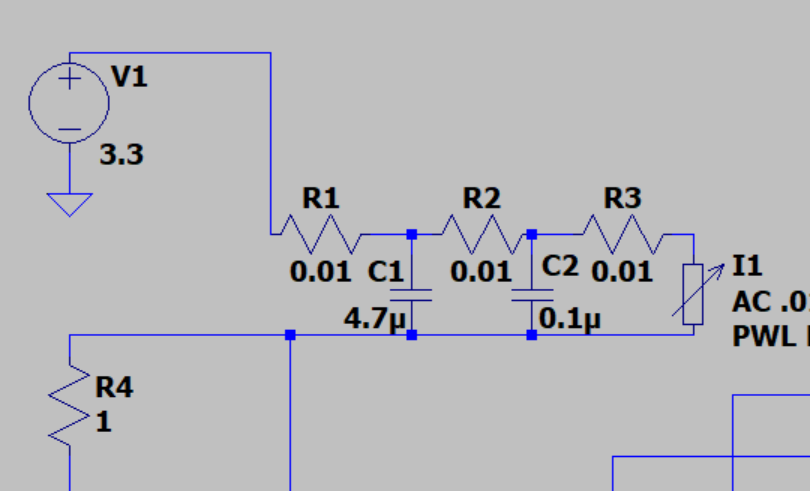
\includegraphics[scale = 0.5]{LPSpice scheme.png}
  \caption{Моделируемая схема}
  \label{ris:LTSpiceScheme}
\end{figure}

\begin{figure}[H]
  \centering
  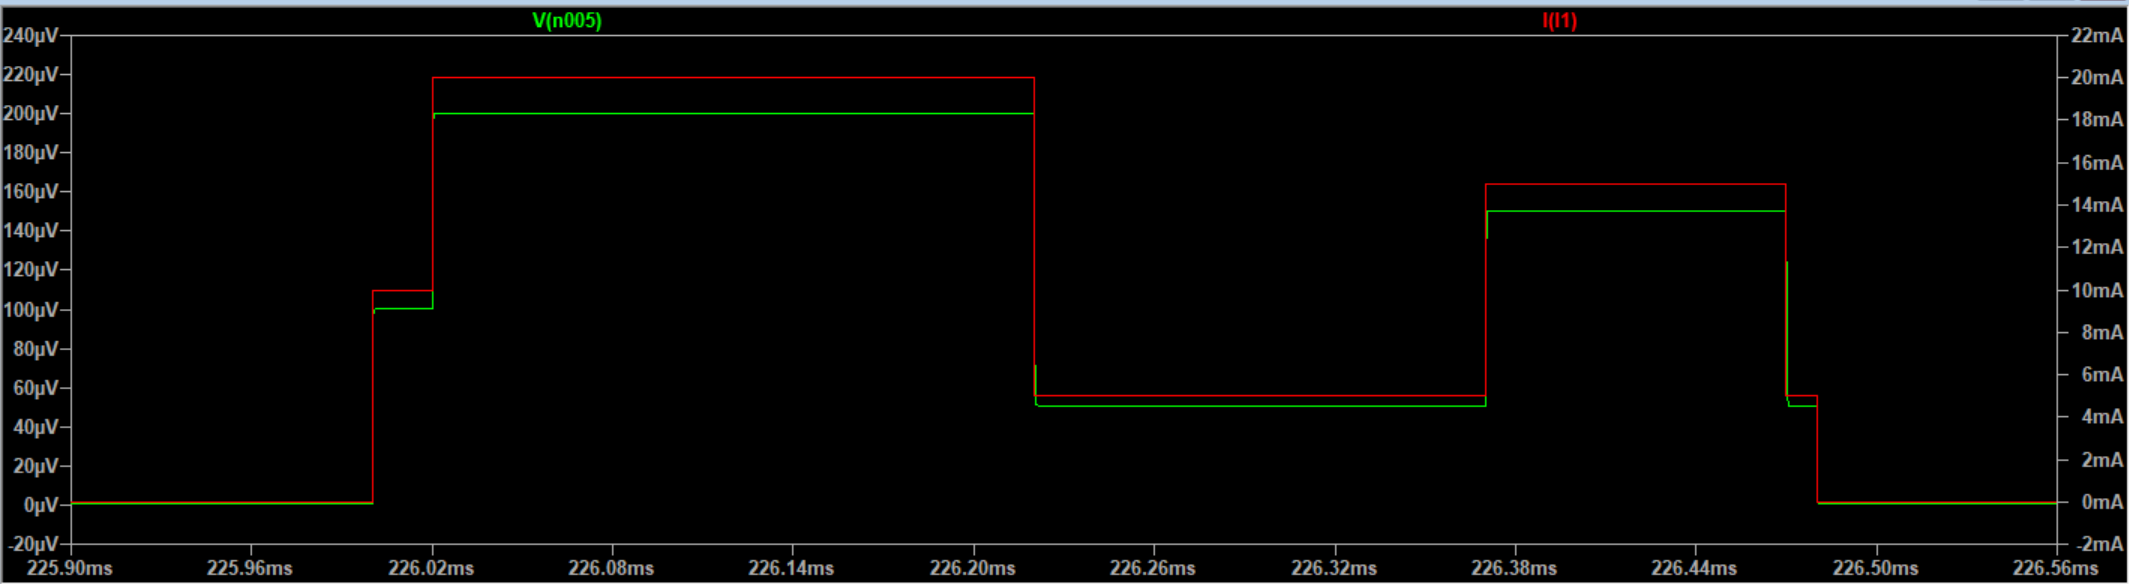
\includegraphics[scale = 0.3]{LTSpice0_01.png}
  \caption{Результаты моделирования амперного диапазона }
  \label{ris:LTSpice0_01}
\end{figure}

Резисторы R1 -- R3 моделируют сопротивления проводников на печатной плате, конденсаторы C1 -- C2 фильтрующие 
по питанию, I1 -- источник тока, моделирующий вышеописанный паттерн поведения BLE-устройства,
R4 - шунт, для амперного диапазона, который равен 0,01 Ом (в дальнейшем в ходе дипломной работы уточняется). 
Красная линия -- входной сигнал, моделирующий потребление отлаживаемого устройства, 
зеленная -- падение напряжения на измеряемом шунте. 

\begin{figure}[H]
  \centering
  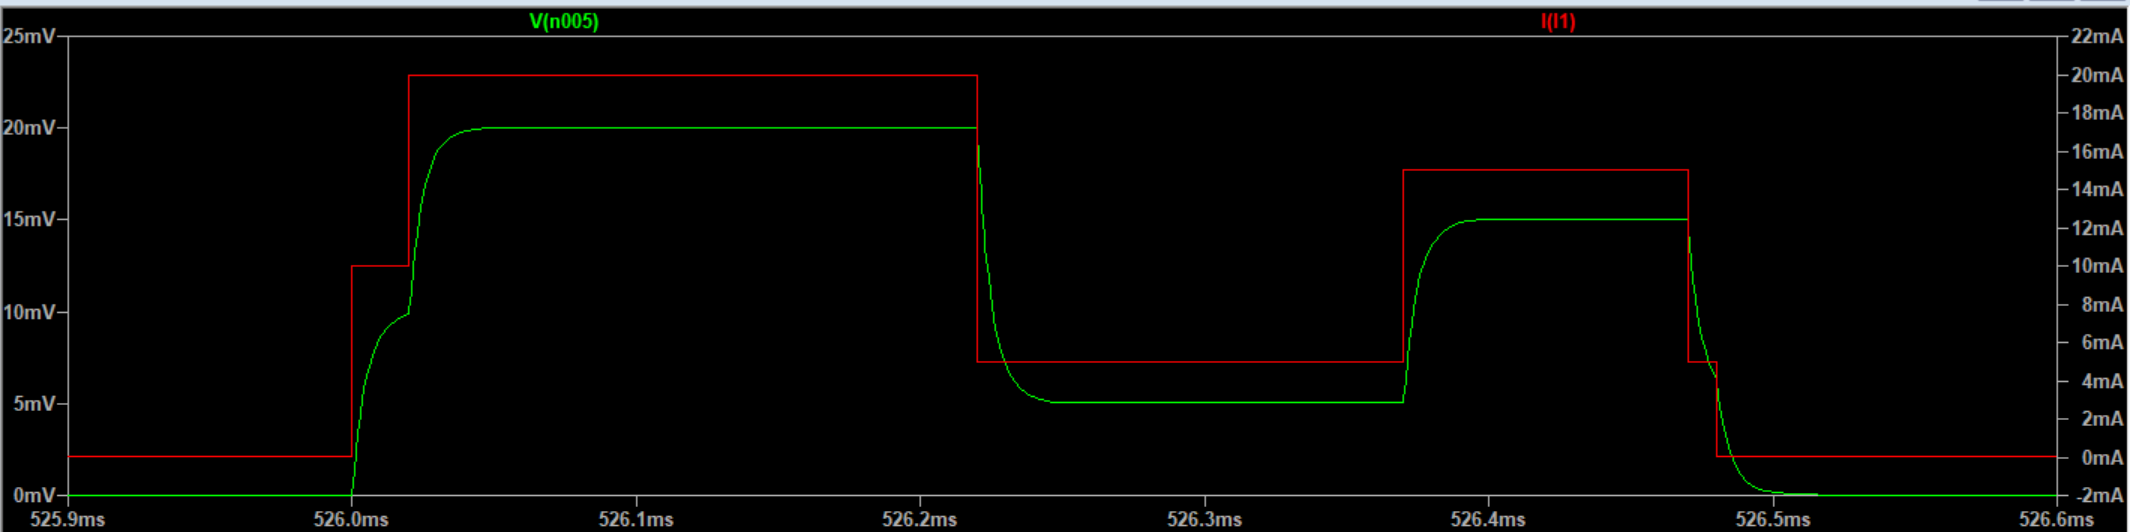
\includegraphics[scale = 0.3]{LTSpice_1.png}
  \caption{Результаты моделирования миллиамперного диапазона }
  \label{ris:LTSpice_1}
\end{figure}

Здесь шунт R4 равен 1 Ом, диапазон -- миллиамперный. 

\begin{figure}[H]
  \centering
  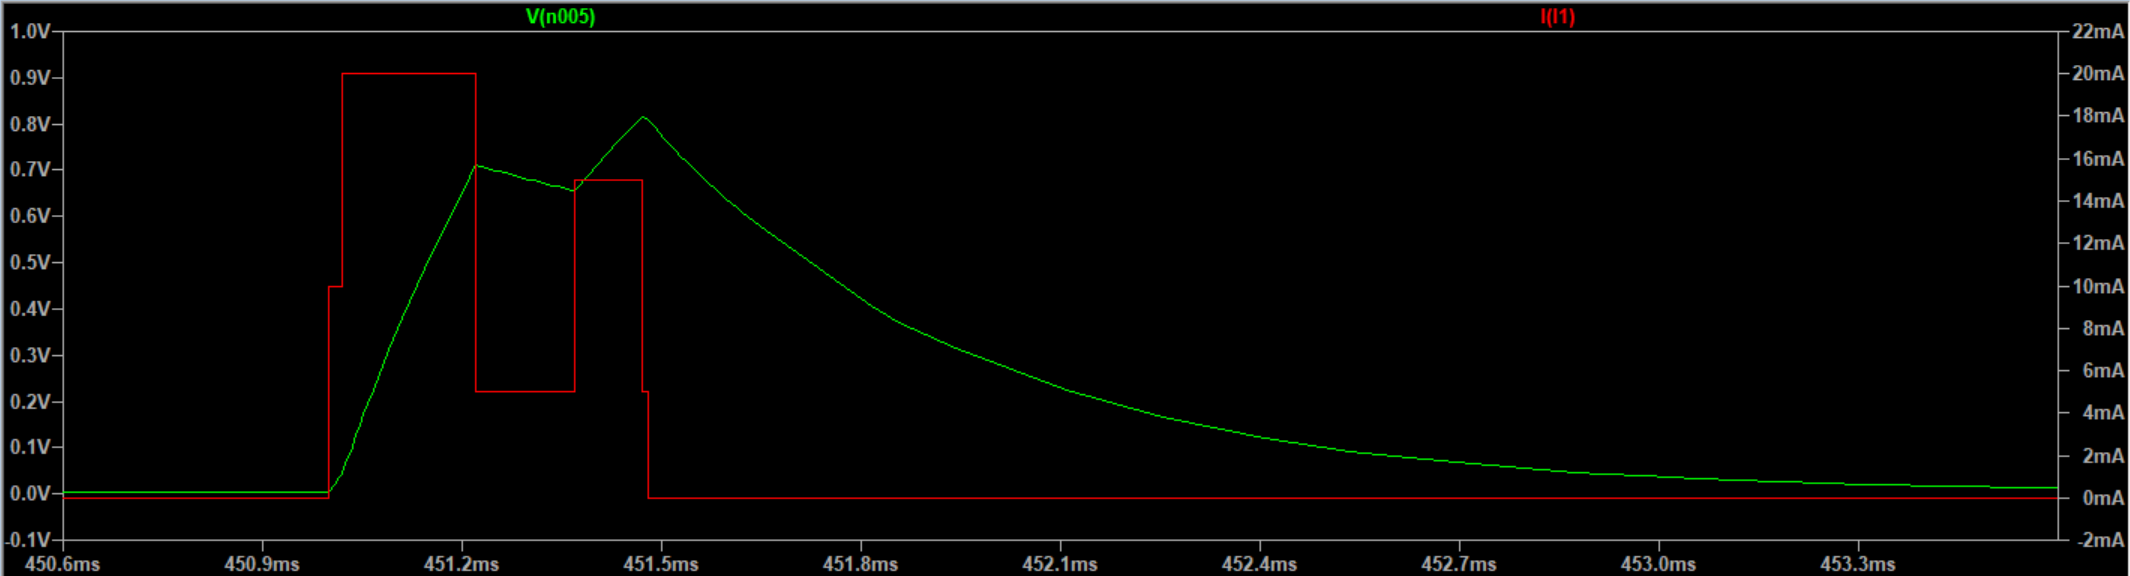
\includegraphics[scale = 0.3]{LTspice100.png}
  \caption{Результаты моделирования микроамперного диапазона }
  \label{ris:LTSpice100}
\end{figure}

А вот моделирование микроамперного диапазона, который можно считать основным измерительным диапазоном для 
IoT-устройств с малым энергопотреблением, показывает, что из-за получившегося из R1 -- R3 и C1 -- C2 RC-фильтра,
уменьшение полосы пропускания на порядки до, примерно, значения в  15 кГц, что определяет требование 
к полосе пропускания.

Так как разрабатываемое устройство является отладчиком, то для <<общения>> с отлаживаемым устройством 
в отладчике должны быть реализованы стандартные для этих целей интерфейсы, такие как UART и отладочные 
SWD/JTAG, что подразумевает под собой наличие удобных, распространенных разъемов. Так же из-за планируемого 
использования в MIEM IoT-LAB, отладчик должен уметь общаться с <<сервером>> по Ethernet, что, по сути,
является требованием заказчика, обусловленное потребностью в возможности гибкого размещения лаборатории на 
территории МИЭМа.  

Для обеспечения конкурентноспособности отладчика, остальные характеристики можно определить 
из таблицы \ref{comparemeasdevices}, а так же из анализа типичной используемой элементной базы.

Резюмируя вышесказанное, можно ориентироваться на следующие требования к разрабатываемому 
устройству:
\begin{itemize}
    \item полоса пропускания -- 15 кГц
    \item напряжение питания отлаживаемых устройств -- от 1,8 В до 12 В
    \item погрешность измерения -- до 5\%
    \item диапазон тока -- от 3,2 мА до 2 А
    \item время переключения диапазонов - десятки мкс
    \item Поддержка Ethernet, UART, SWD/JTAG
    \item себестоимость устройства -- 5000 руб.
\end{itemize}

Данные требования, предъявляемые на этапе начального анализа, в ходе более детальной проработки,
изучения и тестирования в дальнейшем будут уточнены в соответствии с полученными результатами.
% введение

\chapter{Описание структуры устройства}
\section{Подсистема управления}
\hspace{1cm} 

Проектирование любого устройства начинается с определения структуры, которая в дальнейшем
поможет составить его структурную схему. А главным компонентом любого устройства является
его подсистема управления.

Самые популярные подсистемы управления отладчиками базируются на микроконтроллерах,
которые поддерживает основные отладочные интерфейсы -- JTAG и SWD.
В качестве типичного <<отладочного>> микроконтроллера было решено использовать
STM32F107VCT6 из-за его следующих преимуществ \cite{STM32:datasheet}:

\begin{itemize}
    \item \textit{Хорошо проработанная документация} -- компания
     STMicroelectronics является одним из лидеров на рынке микроконтроллеров, во многом благодаря
     замечательной документации, которая позволяет создавать на базе их решений проработанные
     и, по большей части, предсказуемо работающие проекты. Важно быть увереным, что при разработке
     устройства микроконтроллер не начнет показывать <<недокументированные>> возможности и
     различные баги, и репутация компании STMicroelectronics позволяет быть в этом
     уверенным. Антипримером может служить компания Espressif, чьи многочисленные ошибки,
     выявленные после выпуска очередного микроконтроллера, иногда выливаются в довольно
     объемные errata документы.
    \item \textit{Библиотеки} -- наличие удобных и, самое главное, пригодных в использовании 
     библиотек позолит значительно ускорить время разработки. STM32F107VCT6 построена на базе
     ядра Cortex-M3, для которого написано большое количество популярных библиотек, таких
     как HAL, LL, CMSIS, libopencm3 и другие.
    \item \textit{Большое количество готовых решений} -- некоторые из функций разрабатываемой
     системы могли быть реализованы ранее индивидуальным разработчиком, 
     сообществом или предприятием. Разработку всегда стоит начинать с поиска готовых или похожих 
     решений, которые, возможно, уже были разработаны и ждут интеграции в проект. Используемое
     в STM32F107VCT6 ядро сильно повышает шансы найти что-то готовое или то, что сильно 
     ускорит и упростит разработку устройства, позволяя не писать отдельные модули с <<нуля>>.
     \cite{Lakamera:embed}
    \item \textit{Доступность} -- в <<санкционную>> эпоху доступность компонента может стать 
     решающим фактором при выборе. Благодаро своей массовости микроконтроллеры серии STM32 
     можно легко найти как у дистрибьюторов ориентированных на крупные компание, так и на тех,
     кто работает с физическими лицами, что важно в рамках студентческой дипломной работы.
\end{itemize}

\section{Подсистема питания}
\hspace{1cm} 

Невозможно представить устройство без подсистемы питания, которая является его <<сердцем>>,
обеспечивая электроэнергией все остальные подсистемы. Плохо спроектированная система питания
может стать большой проблемой, вплоть до вывода из строя отдельной подсистемы или устройства
вцелом.

В качестве питания для отладчика была выбрана связка из PoE + DC-DC преобразователь, 
выполненный по технологии изолированный fly-back, с возможностью подключения внешнего питания. 

PoE (Power over Ethernet) — это технология передачи удаленным Ethernet-устройствам по 
витой паре электропитания вместе с данными. Данная технология позволяет питать подключенные 
устройства, к которым невозможно или нежелательно проводить кабели для питания.

Технология PoE была выбрана по причине  удобства её использования в устройствах с передачей
данных по Ethernet. Это избавляет от необходимости подключения дополнительных проводов, что
делает отладчик более мобильным. С другой стороны необходимо сохранить возможность подключения
питания более традиционными способами, например через внешний блок питания.

Характеристики различных стандартов PoE представлены в таблице \ref{PoE}.

\begin{table}[H]
    \caption{Основные характеристики стандартов PoE} 
    \label{PoE}
    \begin{center}
    \begin{tabular}{|c|p{2cm}|p{2cm}|p{2cm}|p{2cm}|}
    \hline
  Характеристика/Стандарт & 802.3af  &  802.3at   & 802.3bt & 802.3bt \\ \hline
    Выходная мощность, Вт & 15,4  & 30 А & 60 &  90 \\ \hline
    Мощность на устройстве, Вт & 12,95 & 25,5 & 51 & 71,3  \\ \hline
    Выходное напряжение на источнике, В & 44--57 & 50--57 & 50--57 & 52--57 \\ \hline
    Напряжение на приемнике, В & 37--57 & 42,5--57 & 42,5--57 & 41,1--57  \\ \hline
    Максимальный ток в витой паре, мА & 350 & 600 & 600 & 960  \\ \hline
    \end{tabular}
    \end{center}
\end{table} 

Для понимания какой стандарт PoE будет необходимо реализовать в отладчике
можно оценочно проаннализировать энергопотребление самых энергозатратных элементов устройства.

Максимальная потребляемая мощность микроконтроллера STM32F107VCT6 в корпусе LQFP64 составляет 
444 мВт \cite{STM32:datasheet}, ток потребления выбранного контроллера PoE до 50 мА 
\cite{TPS2376:datasheet}, усредненный ток потребления измерительного операционного усилителя --
до 5 мА, потребляемая мощность выбранной PHY микросхемы до 270 мВт \cite{DP83848:datasheet}.
С учетом усредненного КПД импульсного DC-DC преобразователя, который составляет 70 \%, можно
рассчитывать на то, что мощности 12,95 Вт, которую обеспечивает стандарт 802.3af, должно хватить.

Для маломощных источников питания часто используют fly-back-конверторы, они же обратноходовые
преобразователи. Преимуществами данного решения являются \cite{PowerElectronic:FlyBack}:
\begin{itemize}
  \item Сравнительная простота реализации
  \item Малое количество используемых элементов
  \item Дешевизна
  \item Малая чувствительность к короткому замыканию на выходе
\end{itemize}

Использование же изолированного fly-back преобразователя дает гальваническую развязку по питанию,
что защищает пользователя в случаях случайного касания разъемов, к которым в отладчике 
планируются свободный доступ.

\section{Подсистема измерения энергопотребления}
\hspace{1cm} 

Для измерения тока используется метод снятия напряжения с шунта,
 который представляет собой резистор известного сопротивления с малым отклонением номинала,
 который обычно составляет менее 1\%, с помощью операционного
усилителя, включенного по схеме дифференциального усилителя.
Существует два основных способа подключения измерительной цепи – со стороны никого
или высокого уровня. В ходе производственной практики были рассмотрены и изучены схемы
подключения измерительной цепи по смехе верхнего плеча, которая представлена на рисунке
\ref{ris:231} и по схеме нижнего плеча, которая представлена на рисунке \ref{ris:232}.


\begin{figure}[H]
  \centering
  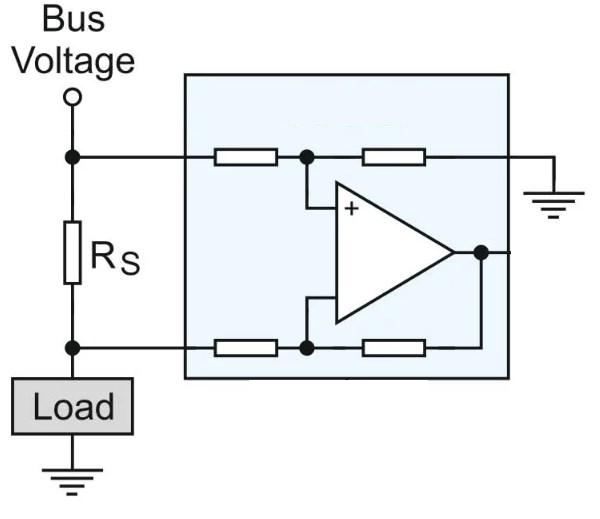
\includegraphics[scale = 0.75]{ris231.png}
  \caption{Схема верхнего плеча}
  \label{ris:231}
\end{figure}

\begin{figure}[H]
  \centering
  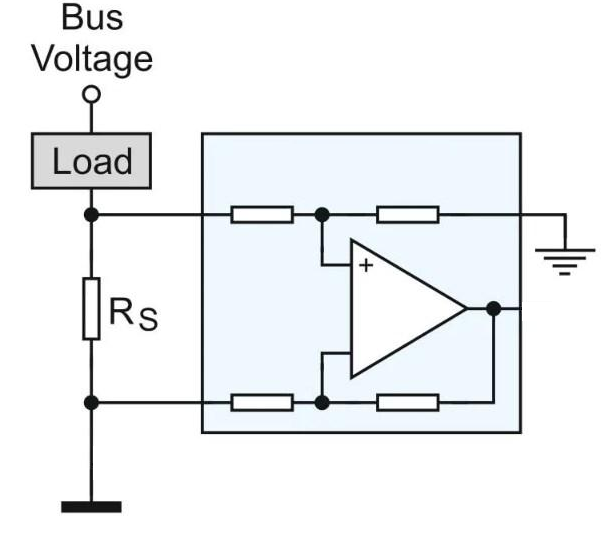
\includegraphics[scale = 0.75]{ris232.png}
  \caption{Схема нижнего плеча}
  \label{ris:232}
\end{figure}

Измерение тока в конфигурации нижнего плеча заключается в размещении измерительного 
элемента между нагрузкой и землей. Этот тип решения довольно легко реализовать, поскольку 
напряжение на измерительном элементе измеряется по отношению к массе цепи. Усилитель 
работает с низкими значениями напряжения (порядка милливольт по отношению к массе схемы), 
что значительно упрощает подбор компонентов и снижает его стоимость.

Основным недостатком этого метода является то, что нагрузка больше не связана напрямую с массой.
 Минусовой вывод нагрузки имеет потенциал на несколько сотен милливольт выше земли, 
 а лучше держать это значение меньше 100 мВ -- эта разница примерно равна падению напряжения
  на шунтирующем резисторе и канале полевого транзистора. Отсутствие прямого соединения
с землей может стать проблемой если в другом месте цепи произойдет короткое замыкание,
    например, если проводящий компонент в устройстве коснется металлического корпуса. 
    Однако для нашего устройства это не будет являться проблемой, так как такой вариант 
    развития событий не предусмотрен.

В случае работы с малыми сигналами довольно большую роль играет входное напряжение 
    смещения усилителя. Чем меньше значение этого параметра, тем выше точность измерения.

Несмотря на эти недостатки, измерение тока на стороне низкого напряжения является хорошим выбором,
 когда нагрузку не нужно подключать напрямую к земле и где нет необходимости обнаруживать 
 короткие замыкания на массу. Но в случае устройств, которые должны соответствовать 
 более строгим требованиям безопасности, измерение тока на стороне высокого 
 напряжения является лучшим выбором.
 После усиления напряжение на выходе ОУ оцифровывается 12-битным АЦП с опорным 
 напряжением 3,3 В, соответственно, каждый значащий разряд АЦП -- это 3,3/4096 = 0,805 мВ.
  При коэффициенте усиления Ку = 50 нашего ОУ, шаг измеряемого напряжения
   на шунте -- около 16 мкВ. Соответственно, при шунтах 100, 1 и 0,01 Ом младшему 
   разряду АЦП соответствует потребляемый ток в 0,16 мкА, 16 мкА и 1,6 мА соответственно 
   \cite{GooglePatent:1}.

\section{Подсистема преобразования уровней}
\hspace{1cm}

Подсистема преобразования уровней нужна для согласования уровней и изоляции от паразитного 
питания шин с разным напряжением. Подсистема будет согласовывать уровни напряжения между
отлдачиком и отлаживаем устройством по линиям передачи данных. 

Надежным и быстрым решением будет использование специализированной микросхемы 74LVC2T45, из-за
следующих преимуществ \cite{SN74LVC2T45:datasheet}:
\begin{itemize}
  \item Работает во всем диапазоне напряжений от 1,65 В до 5,5 В
  \item Имеет функцию изоляции напряжения питания отлаживаемого устройства переводом каналов в
  высокоимпедансное состояние
  \item Малый ток потребления -- до 4 мкА
  \item Минимальная скорость передачи данных 75 Мбит/с
  \item Имеет защиту от статики в соответствии со стандартом JESD20
\end{itemize}
 Ее функциональная диаграмма изображена на рисунке \ref{ris:241}.

\begin{figure}[H]
  \centering
  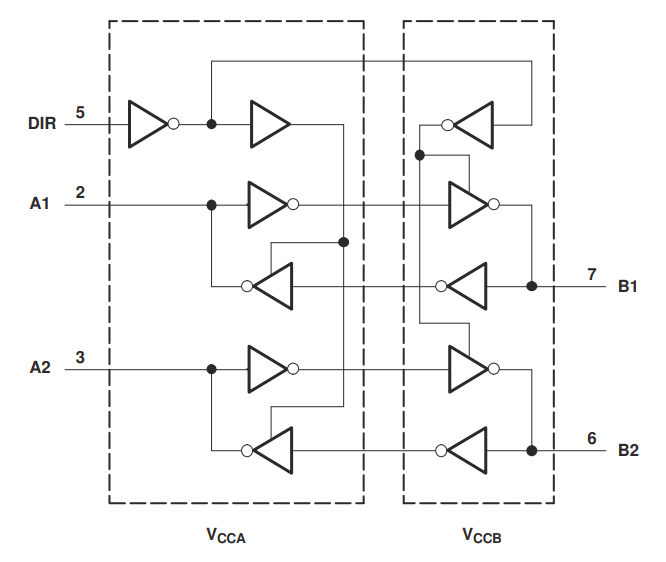
\includegraphics[scale = 0.75]{ris241.png}
  \caption{Функциональная схема 74LVC2T45}
  \label{ris:241}
\end{figure}


\section{Подсистема Ethernet}
\hspace{1cm}

Данная подсистема будет состоять из входного безтрансофрматорного разъема типа RJ-45, 
согласующего трансформатора, и PHY-микросхемы, предназначеной для выполнения функций 
физического уровня сетевой модели OSI.

Связка из безтрансофрматорного разъема и согласующего трансформатора отдельной
микросхмеой была выбрана для совместимости с PoE, так как большинство доступных разъемов со 
встроенным трансмофрматором не имеют отводов от средней точки трансформатора со стороны кабеля,
что необходимо для работы PoE. 

На рисунке \ref{ris:251} изображена внутренняя структура согласующего трансформатора на примере микросхемы
HX1188NL. Проблема у большинства разъемов со встроенным трансформаторо возникала из-за
отсутствия связей 2 и 7. 

\begin{figure}[H]
  \centering
  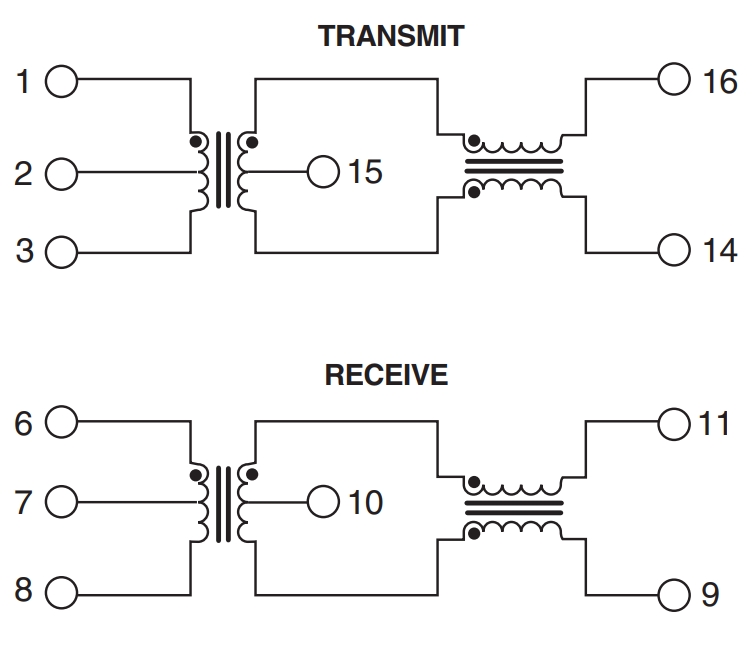
\includegraphics[scale = 0.75]{ris251.png}
  \caption{Внутренняя структура HX1188NL}
  \label{ris:251}
\end{figure}

В качестве Ethernet-контроллера была выбрана микросхема DP83848-EP из-за того, что при отладке
прошивки использовалась отладочная плата именно с этой PHY-микросхемой <<на борту>>. Использование
другой микросхемы привело бы к увелечению времени отладки устройства и более глубокой переработки
уже готового решения, что нерационально.

\section{Структурная схема устройства}
\hspace{1cm}

Исходя из всего вышесказанного, можно составить структурную схему устройства, которая изображена
на рисунке \ref{ris:261}.

\begin{figure}[H]
  \centering
  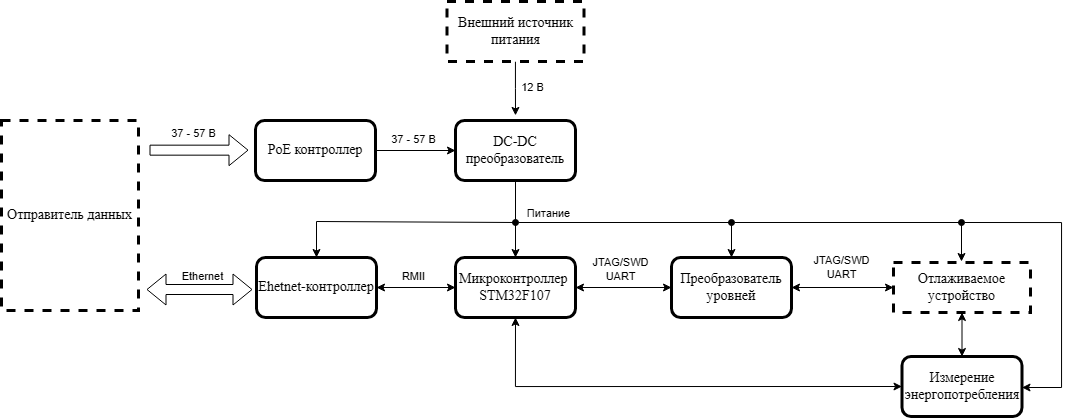
\includegraphics[scale = 0.48]{ris261.png}
  \caption{Структурная схема устройства}
  \label{ris:261}
\end{figure}

Здесь в качестве отправителя выступает условное устройство, от которого будут приходить
команды по Ethernet, PoE-контроллер и DC-DC преобразователь вместе составляют подсистему питания,
Ethernet-контроллер является подсистемой Ethernet, STM32F107 -- подсистема управления, 
преобразователь уровней является подсистемой преобразования уровней, измерение энергопотребления --
это одноименная подсистема, а отлаживаемое устройство представляет собой целевой микроконтроллер,
на который будет отправляться прошивка и чье энергопотребление будет измеряться.

%В случае нехватки объема добавить разгон про модель OSI

%В измерительных приборах вопрос питания стоит особенно остро, ведь даже те помехи, которые 
%не нанесли бы обычному цифровому устройству значительного вреда, могут с легкостью испортить
%всю точность измерения -----------сильная заготовка, но в другую главу-------------
 % описание структуры устройства
\chapter{Описание принципа работы подсистемы питания}
\section{Описание схемотехнического решения}
\subsection{PoE-контроллер}
\hspace{1cm} 

В измерительных приборах вопрос питания стоит особенно остро, ведь даже те помехи, которые 
не нанесли бы обычному цифровому устройству значительного вреда, могут с легкостью испортить
всю точность измерения измерительных аналоговых частей приборов. Поэтому грамотный и продуманный расчет 
подсистемы питания, основанный на опыте крупных компаний -- залог правильной и предсказуемой работы устройства.
Именно по этой причине за основу самого критического узла питания отладчика -- DC-DC преобразователя,
было взято решении компании Texas Instruments.
Подсистема питания состоит из трех частей:

\begin{enumerate}
    \item Микросхема контроллера PoE TPS2376 с обвязкой.
    \item DC-DC преобразователь LMR36520FADDA с обвязкой.
    \item LDO стабилизатор TLV1117 с обвязкой.
    \item Понижающий ШИМ-регулятор  ST1S10.
\end{enumerate}

За основу схемотехнического решения контроллера PoE взята типичная применяемая схема для
микросхемы TPS2376, которая была доработана и изображена на рисунке \ref{ris:311}.

\begin{figure}[H]
    \centering
    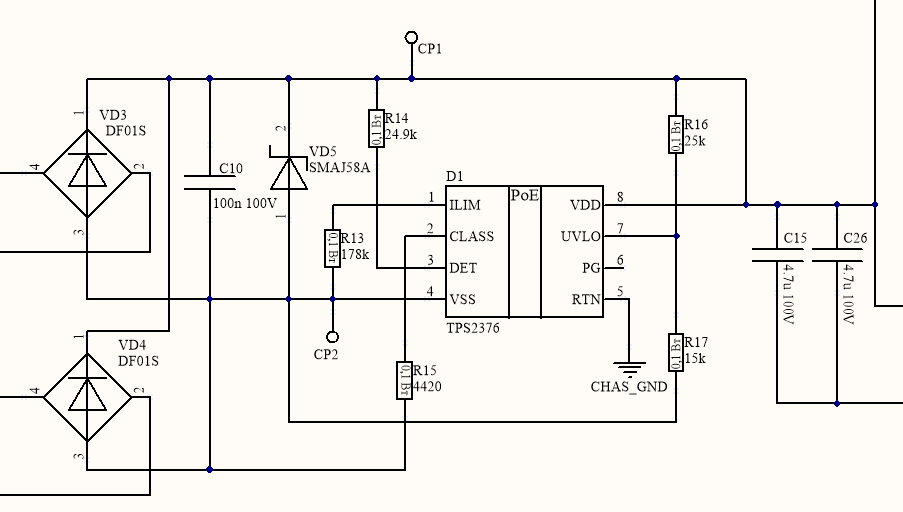
\includegraphics[scale = 0.7]{ris311.png}
    \caption{Принципиальная электрическая схема обвзяки TPS2376 }
    \label{ris:311}
\end{figure}

На четвертый контакт диодного моста VD3 приходит сигнал с четвертого и пятого контактов 
Ethernet-разъема RJ45, которые отвечают за подключение отрицательного напряжения PoE.
На второй контакт диодного моста VD3 приходит сигнал с седьмого и восьмого контактов 
Ethernet-разъема RJ45, которые отвечают за подключение положительного напряжения PoE.  
На второй и четвертый контакты диодного моста VD4 приходят сигналы со средней точки согласующего
Ethernet-трансформатора с линий передачи и приема данных. Диодные мосты нужны для защиты последующей 
части устройства от различного исполнения разъема RJ-45, в случае если вдруг контакты положительного 
и отрицательного напряжения PoE будут поменяны местам.

Керамический конденсатор C10 является фильтрующим по питанию. Фильтрующие конденсаторы предназначены 
для фильтрации питания микросхем от высокочастотных помех и обычно их номинал равень 100 нФ.
Такие конденсаторы встречаются довольно  часто, и в дальнейшем в этой дипломной работе не будет 
описываться их назначение. Так как максимальное напряжение PoE 57 В, то рабочее напряжение 
конденсатор C10 выбрано почти с двойным запасом для повышения срока службы и надежности схемы.

Супрессор VD5 предназначен для защиты микросхемы от перенапряжения, например в случае поражения
линии статикой и расчитан на рабочее напряжение в 58 В. 

Резистор R13 предназначен для ограничения пускового тока. Ограничение пускового тока ограничивает
протекание тока через выходные конденсаторы C15 и С26 в начальный момент их зарядки и не дает 
вызвать просадку напряжения ниже, чем задает делитель напряжения R16, R17 на выводе UVLO. 
Рекомендумый номинал резистора -- 178 кОм.  

Обычно сопротивление резистора R14 должно быть равно 24,9 кОм. Rdet подключен к входной линии, 
когда VDD находится в диапазоне от 1,4 В до 11,3 В, и отключается,
когда напряжение на линии выходит за пределы этого диапазона, чтобы сэкономить энергию.
Этот диапазон напряжений был выбран для того, чтобы обеспечить возможность обнаружения с 
помощью двух кремниевых выпрямителей между контроллером PoE и разъемом RJ-45.

Значение резистора R15 было выбрано равным 4420 Ом исходя из 
необходимой выходной мощности по таблице \ref{ClassTPS2376} \cite{TPS2376:datasheet}.

\begin{table}[H]
    \caption{Классификация TPS2376} 
    \label{ClassTPS2376}
    \begin{center}
    \begin{tabular}{|c|c|c|c|}
    \hline
    Class & PD POWER, W  &  Rclass, Ohm   & 802.3af LIMITS, mA \\ \hline
    0 & 0,44 -- 12,95  & 4420 &0 -- 4  \\ \hline
    1 & 0,44 -- 3,84 & 953 & 9 -- 12   \\ \hline
    2 & 3,84 -- 6,49 & 549 & 17 -- 20  \\ \hline
    3 & 6,49 -- 12,95 & 357 & 26 -- 30   \\ \hline
    \end{tabular}
    \end{center}
\end{table} 

Вывод VSS подключается к минусу выходного с диодных мостов напряжения, 
а вывод VDD подключается к плюсу этого напряжения.

Вывод PG предназначен для передачи разрешающего сигнала на работу последующих микросхем,
в данной схеме нет потребности в реализации дополнительных условий или задержек включения
дальнейших элементов схемы, поэтому он не используется.

Вывод UVLO используется с внешним резисторным делителем между VDD и VSS для установки 
верхнего и нижнего порогов UVLO. TPS2376 включает выход, когда напряжение UVLO превышает верхний 
порог UVLO. Когда начинает течь ток, VDD проседает из-за сопротивления кабеля и динамического 
сопротивления входных диодов. Нижний порог UVLO должен быть ниже самого низкого напряжения, 
которого достигает вход. Коэффициент делителя должен быть выбран таким образом, 
чтобы получить примерно 21 В на выводе UVLO, когда VDD находится на требуемом 
напряжении включения. Поэтому R16 и R17 выбраны номиналом 25 кОм и 15 кОм соответственно.

Выходные конденсаторы С15 и С26 предназначены для фильтрации выходного напряжения, но взяты 
несколько меньше по номиналу рекомендуемых для уменьшения габаритов устройства. Их рабочее
напряжение так же взято с почти двойным запасом \cite{TPS2376:datasheet}.

Общий принцип работы этого в обеспечении стандрата IEEE 802.3af, который определяет 
процесс безопасного питания по PoE по Ethernet-кабелю и последующего отключения питания, 
если нагрузка отсоединена. Процесс проходит через три рабочих состояния: обнаружение, 
классификация и работа. Смысл процесса заключается в том, что когда нагрузка не подключена,
контроллер PoE периодически проверяет наличие подключенного устройства -- это называется 
обнаружением. Если подключается нагрузка, то контроллер может запросить информацию о том,
сколько энергии она потребует -- это этап классификации. Знание потребности в мощности нагрузки 
позволяет контроллеру PoE разумно отдавать и распределять энергую, в случае нескольких нагрузок,
а так же защищать себя от перегрузки. После этапа классификации контроллер подает питание на 
нагрузку и контролирует линию питания на предмет перегрузки. Если после этого отключить нагрузку,
контроллер снова войдет в исходное состояние обнаружения. Рисунок \ref{ris:312}  илюстрирует 
вышеописанный паттерн поведения контроллера PoE \cite{TPS2376:datasheet}.

\begin{figure}[H]
    \centering
    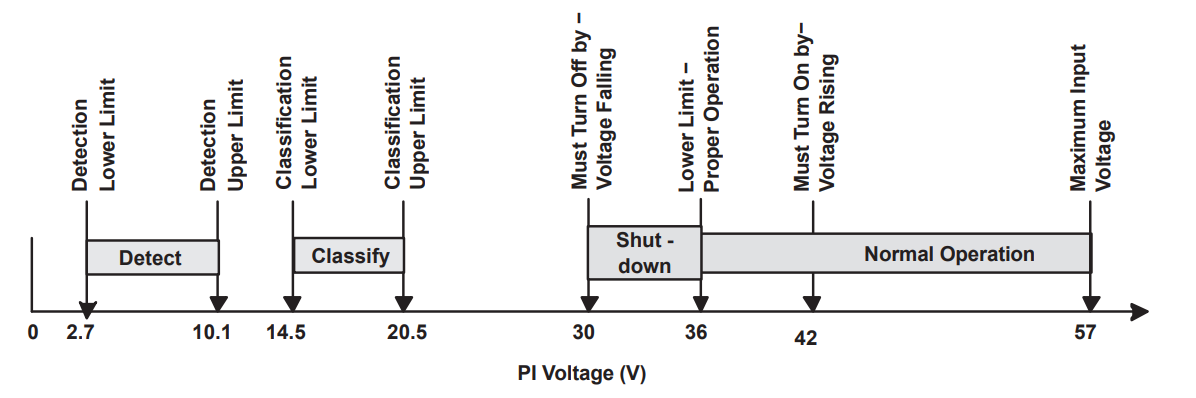
\includegraphics[scale = 0.55]{ris312.png}
    \caption{IEEE 802.3 PD Limits}
    \label{ris:312}
\end{figure}

Ожидаемые осциллограммы в основных узлах этой части схемы представлены на рисунке 
\ref{ris:313} \cite{TPS2376:datasheet}.

\begin{figure}[H]
    \centering
    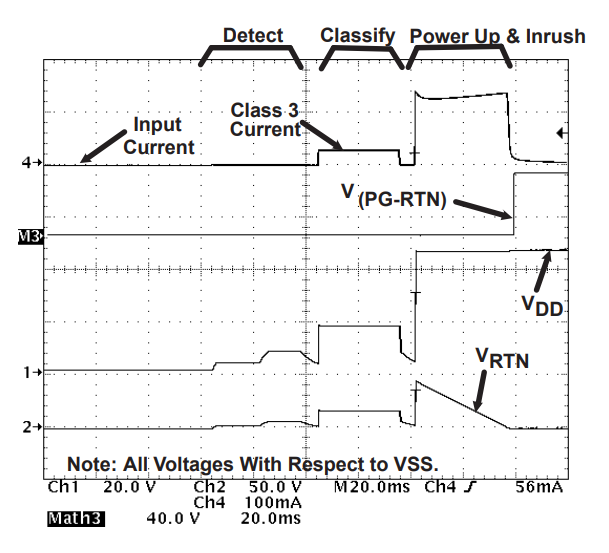
\includegraphics[scale = 0.75]{ris313.png}
    \caption{Осциллограммы TPS2376 при включении}
    \label{ris:313}
\end{figure}

\subsection{DC-DC преобразователь}
\hspace{1cm} 

В качестве изолированного Fly-Buck-преобразователя было выбрано решение на базе микросхемы LMR36520 
от компании Texas Instruments из-за наличия подробной документации по расчету каждого элемента
обвязки. 

Схемотехническое решение представлено на рисунке \ref{ris:321}.

\begin{figure}[H]
    \centering
    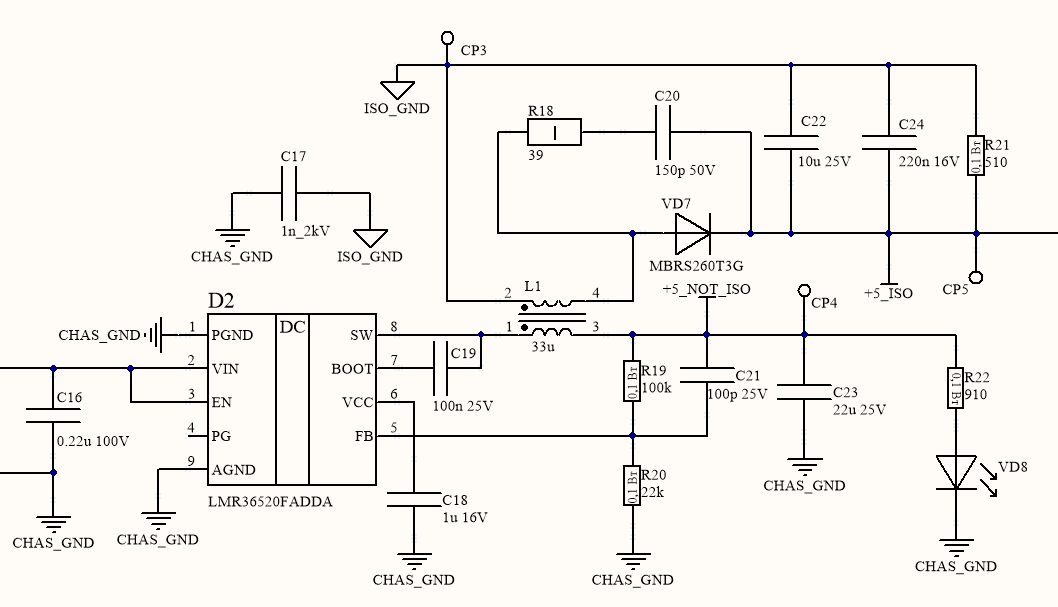
\includegraphics[scale = 0.65]{ris321.png}
    \caption{Принципиальная электрическая схема обвязки LMR36520}
    \label{ris:321}
\end{figure}

Конденсатор С16 является фильтрующим по входному питанию.На вывод VIN приходит напряжение
с выхода PoE-контроллера. Сигнал EN является разрешающим работу преобразователя. Так как
в данной схеме нет потребности в реализации дополнительных условий или задержек включения
DC-DC преобразователя, то этот вывод останется неподключеным. PGND и AGND соединены внутри 
микросхемы и подключаются к <<аналоговой>> земле. 

PG -- это выход флага состояния питания преобразователя, является выходом с открытым стоком. 
В данной схеме нет потребности в отслеживании включения преобразователя, поэтому этот вывод не 
используется. 

FB -- вход обратной связи регулятора, подключается к средней точки резистивного делителя
напряжения.

Вывод VCC является выходом внутреннего стабилизатора на 5 В, для <<собственных нужд>> преобразователя.

К выводу BOOT подключается bootstrap конденсатор, он же конденсатор запуска, номиналом 100 нФ 
\cite{LMR36520:datasheet}. 

Индуктивность L1 выполняет роль накопителя энергии в FlyBack-преобразователях.
Для описания их работы рассмотрим схему замещения, изображенную на рисунке \ref{ris:322}.

\begin{figure}[H]
    \centering
    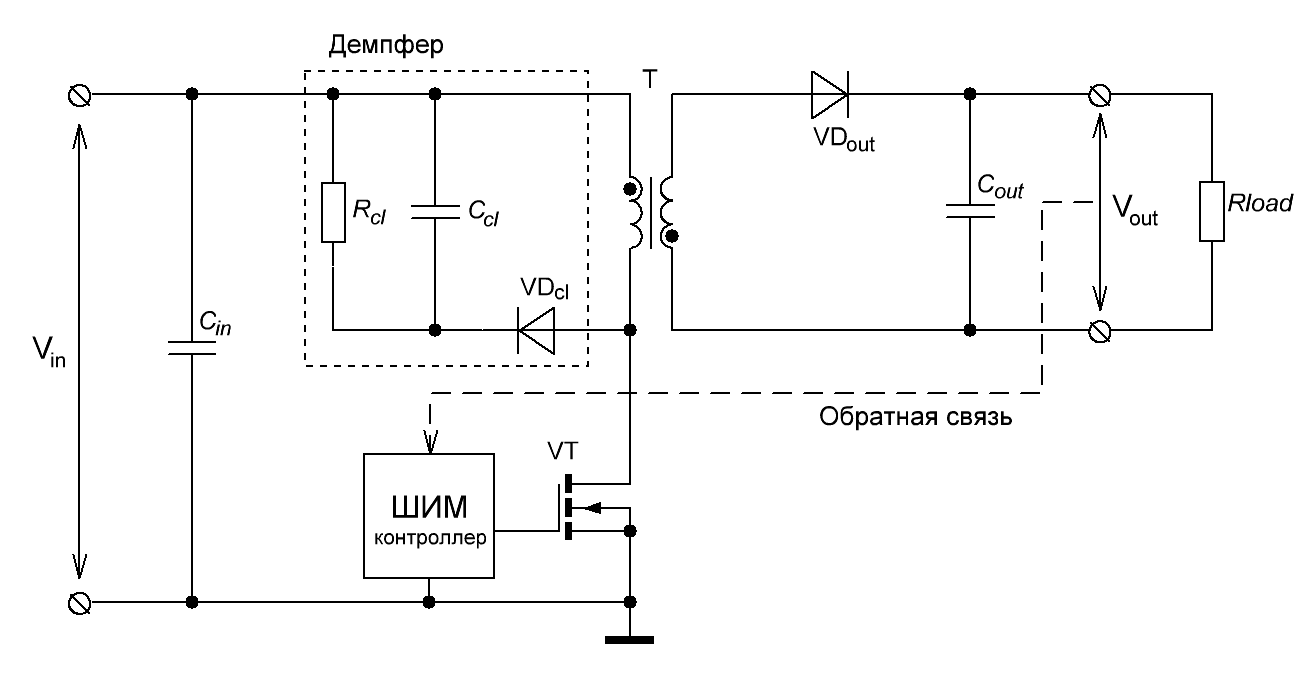
\includegraphics[scale = 0.5]{ris322.png}
    \caption{Упрощенная электрическая схема обратноходового преобразователя}
    \label{ris:322}
\end{figure}

Принцип работы обратноходового преобразователя состоит в следующем. Ключевой транзистор, 
управляемый ШИМ-контроллером, которые в рамках нашего схемотехнического решения встроены
в микросхему LMR36520, коммутирует первичную обмотку трансформатора к источнику питания.
Первичная обмотка обратноходового трансформатора фактически представляет собой дроссель, 
поэтому после коммутации ток через неё линейно растет и энергия накапливается в магнитопроводе. 
К выходному диоду приложено запирающее напряжение и ток во вторичной обмотке не протекает. 
В момент, когда транзистор закрывается, полярность на обмотках в соответствии с законом 
самоиндукции изменяется на противоположную. Диод открывается, ток начинает протекать через
вторичную обмотку трансформатора, и энергия, запасенная в магнитопроводе, переходит в нагрузку. 
И это при закрытом ключе. Далее процесс повторяется. Выходной конденсатор фильтра является 
энергетическим буфером, поддерживающем ток в нагрузке в моменты паузы.
В основе работы преобразователя лежит накопление энергии в индуктивности первичной обмотки 
на первой во времени стадии заряда и передача запасенной энергии на последующей стадии 
передачи энергии. Поскольку стадии накопления и передачи энергии разделены во времени, 
то трансформатор в обратноходовом преобразователе фактически представляет собой индуктивностью 
с двумя или более обмотками. Этот факт Мы используем для уменьшения габаритов схемы и ее упрощения,
заменив трансформатор в нашем преобразователе на две взаимосвязанные катушки индуктивности в 
одном корпусе -- L1, образуя трансформатор с коэффициентом трансформации равным единице
\cite{PowerElectronic:FlyBack} 
\cite{Würth Elektronik:Application Note}
\cite{DC-DC_Book:Recom}.

Вернемся к рассмотрению рисунка \ref{ris:321}. В качестве выходных конденсаторов используются
С23 для неизолированного выхода и С22, С24 для изолированного выхода. В качестве демпферной цепи 
выступают R18, C20 и VD7. Светодиод VD8 и его токоограничительный резистор R22 служат для 
индикации питания. Конденсатор C17 используется для защиты от статики в случае прикосновения ко 
входному разему RJ-45, образуя емкостной делитель с прикоснувшимся человеком, снижая амплитуду 
выброса статического напряжения. 

\subsection{LDO стабилизатор}
\hspace{1cm}

Микросхема TLV1117 представляет собой положительный стабилизатор напряжения с низким падением напряжения, 
способный обеспечить выходной ток до 800 мА. Схема обвязки изображена на рисунке \ref{ris:324}: 

\begin{figure}[H]
    \centering
    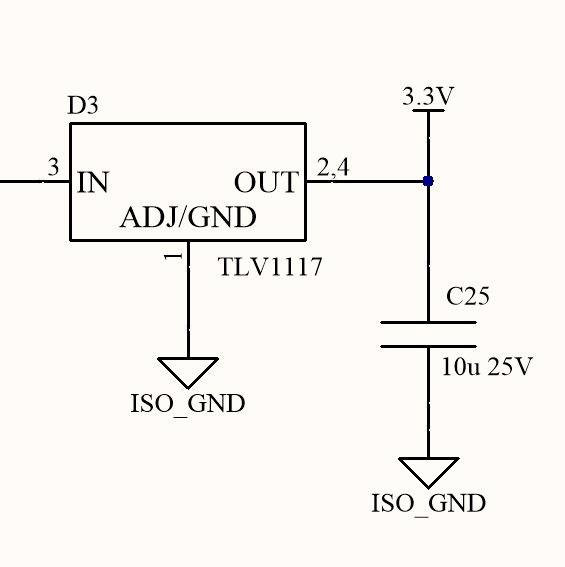
\includegraphics[scale = 0.6]{ris324.png}
    \caption{Схемотехническое решение на базе TLV1117}
    \label{ris:324}
\end{figure}

Отсутствие входной емкости обусловлено достаточным уровнем фильтрации сигнала на изолированном выходе 
DC-DC преобразователя, выходная емкость была выбрана значением 10 мкФ в соотвествии с документацией 
на стабилизатор \cite{TLV1117:datasheet}. 

\subsection{Источник питания преобразователя уровней}
\hspace{1cm}

В качестве источника питания преобразователя уровней или отлаживаемых устройств (опционально) было решено 
использовать понижающий ШИМ-регулятор ST1S10, который способен обеспечить выходной ток до 3 А. 
Применяемая нами схема с его участием изображена 

на рисунке \ref{ris:ST1S10}

\begin{figure}[H]
    \centering
    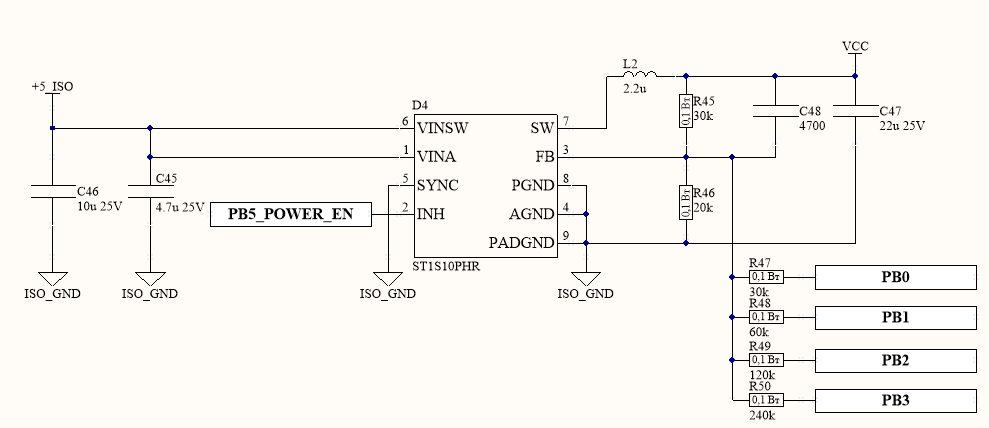
\includegraphics[scale = 0.7]{ST1S10 scheme.png}
    \caption{Схемотехническое решение на базе ST1S10}
    \label{ris:ST1S10}
\end{figure}

Здесь вывод VINSW предназначен для подачи входного напряжения питания, к нему подключается фильтрующий 
конденсатор C46. Вывод VINA -- для подачи входного аналогового напряжения, которому так же подключается 
фильтрующий конденсатор. 

Вывод INH являюется запрещающим, с активным низким уровнем, на него подается сигнал запрета работы от 
микроконтроллера. 

Если вывод SYNC подключен к земле, то регулятор работает на частоте 900 кГц, в иных случаях к этому выводу 
следует подключать внешний кварцевый генератор с тактовой частотой от 400 кГц до 1,2 МГц. В нашей схеме 
будем использовать частоту работы по умолчанию -- 900 кГц, подключив SYNC к земле. 

Выводы PGND, AGND, PADGND в нашей схеме подключаются к земле. 

С вывода SW снимается выходной ШИМ-сигнал, который подается на индуктивность L2, которая вместе с 
выходной емкостью C47 образуют LC-фильтр нижних частот, который выпрямляет ШИМ с SW. 

Для возможности подключения емкостной нагрузки значением более чем 100 мкФ необходимо добавить в схему 
конденсатор C48 с номиналом 4,7 нФ. 

Резисторы R45 -- R50 образуют делитель напряжения, средняя точка которого приходит на вывод FB, тем самым 
обеспечивая регулировку выходного с ST1S10 напряжения. 

Выходное напряжение расчитывается по формуле \ref{eq:VoutST1S10}

\begin{equation}
    V_{out} = \frac{R45 \cdot 0,8}{R46 || r} + 0,8 
    \label{eq:VoutST1S10}
\end{equation}

, где r -- сопротивление одного из резисторов R47, R48, R49, R50 или ни одного из них, 
в зависимости от управляющих сигналов, поступивших с выводов микроконтроллера  PB0, PB1, PB2, PB3 
соответственно. Такая регулирвоака повзоляет за счет отключения или подкючения резисторов управлять 
выходным напряжением с ST1S10 в диапазоне от 2 В -- случай когда ни один из резисторов не подключен к 
выводу FB, до 2,8 В, в случае когда подключен резистор R47 \cite{ST1S10:datasheet}. 


\section{Расчет элементов схемы}
\subsection{Исходные данные}
\hspace{1cm} 

Перед расчетом элементов обвязки DC-DC преобразователя следует определиться с исходными данными:

\begin{itemize}
    \item Диапазон входных напряжений от $U_{in.min.}$ = 12 В, что соответсвтует напряжению
    внешнего источника питания, до $U_{in.max}$ = 57 В, что соответсвтует максимальному
    напряжению с выхода контроллера PoE. 
    \item Частота ШИМ-контроллера, встроенного в LMR36520 равна $f_{sw}$ = 400 кГц 
    \cite{LMR36520:datasheet}. 
    \item Выходное напряжение на неизолированном выходе $U_{out1}$ = 5,5 В, максимальынй 
    выходной ток этого выхода примем $I_{out1}$ = 50 мА для подключения светодиода и запаса 
    , который может понадобиться в ходе доработок и отладки устройства. 
    \item Выходное напряжение на изолированном выходе $U_{out2}$ = 5,5 В, но с возможностью допуска
    до 6,5 В из-за того, что это напряжение подается на преобразователь 3,3 В, который допускает 
    такое входное напряжение. Максимальный ток изолированного выхода примем равным $I_{out2}$ = 1 А,
    что обусловлено потребляемым током Wi-Fi решений и сотовых модемов в пике во время передачи 
    данных. 
    \item Падение на диоде VD7 примем равным $U_{f}$ = 0,5 В - типичное для выпрямительных диодов Шоттки, 
    в дальнейшем, при подобе диода, уточним его.
    
\end{itemize}

\subsection{Расчет индуктивности}
\hspace{1cm} 

Коэффициент трансформации $dN$ расчитывается по формуле \ref{eq:dN}:

\begin{equation}
    dN = \frac{U_{out2} + U_{f}}{ U_{out1}} = \frac{5,5 + 1}{5,5} = 1,091
    \label{eq:dN}
\end{equation}

Из формулы \ref{eq:dN} видно, что если взять связанные индуктивности с коэффициентом 
трансформации равным 1, то это будет допустимой потерей точности расчетов. 

Далее введем минимальный коээффициент заполнения ШИМ $D_{min}$, который расчитывается по 
формуле \ref{eq:Dmin}:

\begin{equation}
    D_{min} = \frac{U_{in.min}}{U_{in.max}} = \frac{12}{57} = 0,096
    \label{eq:Dmin}
\end{equation}

А максимальный коэффициент заполнения ШИМ равен $D_{max}$ = 0,5, что обуславливается внутренними
конструктивными ограничениями LMR36520. Коэффициенты заполнения показывают степень зарядки 
катушки индуктивности, чем больше $D$, тем больше успеет запастись энергии в катушке, для дальнейшей
передачи на выход схемы, и наоборот, чем меньше коэффициент заполнения, тем энергии будет меньше. 

Индуктивность катушки расчитывается по формуле \ref{eq:L}:

\begin{equation}
    L =
    (U_{in. max} \cdot U_{out1}) \cdot \frac{D_{min}}{\Delta i \cdot f_{sw}} = 
    57 \cdot 5,5 \cdot \frac{0,096}{0,35 \cdot 400000} =
     3,549 \cdot 10^{-5}  \text{ Гн,}
    \label{eq:L}
\end{equation}

где $\Delta i$ отражает пиковую пульсацию тока намагничивания и устанавливатся
в диапазоне от 30\% до 40\%. Было взято среднее значение в 35\%. 

Получившуюся по формуле \ref{eq:L} индуктивность L1 выберем ближайшей из доступного номинала 
индуктивностей серии MSD1278, компании CoilCraft \cite{MSD1278:datasheet}. Получилось, что L1 = 33 мкГн. 

Поскольку ток намагничивания совпадает с типичной формой тока дросселя, мы можем рассчитать пульсации 
тока от пика до пика $\varDelta i_{m}$, используя уравнение \ref{eq:dIm}

\begin{equation}
    \varDelta i_{m} =
    \frac{(U_{in.max} - U_{out1}) \cdot D_{min}}{L \cdot f_{sw}} =
    \frac{(57 - 5,5) \cdot 0,096}{33 \cdot 10^{-6} \cdot 400000} =
    0,376 \text{ А}
    \label{eq:dIm}
\end{equation}

Далее нужно оценить пиковые значения положительного и отрицательного токов выбросов при переключении
управляющего транизстора, который встроен в микросхему LMR36520. 

Пиковый положительный ток выброса $I_{pospk}$ расчитывается по формуле \ref{eq:Ipospk}:

\begin{equation}
    I_{pospk} =
    I_{out1} + (dN \cdot I_{out2}) + \frac{\Delta i_{m}}{2} = 
    0,05 + (1 \cdot 1) + \frac{0,376}{2} =
    1,238
    \label{eq:Ipospk}
\end{equation}

Ограничение на положительный пиковый ток задается внутренним строенимем LMR36520 и равно 2,4 А, что больше
полученных нами 1,234 А при расчетах. 

Исходя из ограничения на отрицательный пиковый ток, равное -1,7 А, уравнение \ref{eq:Ioutmax} задает 
максимальный выходной ток изолированного выхода.

\begin{equation}
   I_{out2.max} = \frac{(1,7 - \frac{\Delta i_{m}}{2} + I_{out2}) \cdot (V_{in} - V_{out1})}{2 \cdot V_{out2}}
\label{eq:Ioutmax}
\end{equation}


При входном напряжении равным 12 В по формуле \ref{eq:Ioutmax} получается, что $I_{out2.max}$ = 0,923, 
что меньше заданного нами одного ампера. Однако, при входном напряжении равным 12,6 В 
$I_{out2.max}$ = 1,008 А, что уже нам подходит. \cite{LMR36520:Aplication Note}. 

\subsection{Расчет выходной емкости неизолированного выхода}
\hspace{1cm} 

Рекомендуемое значение емкости выходного конденсатор расчитывается по формуле \ref{eq:Cout1}:

\begin{eqnarray}
    C_{out1} =
    \frac{\Delta I_{out1}}{f_{sw} \cdot \Delta U_{out1} \cdot K} \cdot 
    [(1 - D_{min}) \cdot (1 + K) + \frac{K^{2}}{12} \cdot (2 - D_{min})] = \nonumber\\
    \frac{0,05}{400000 \cdot 0,05 \cdot 0,4} \cdot 
    [(1 - 0,115) \cdot (1 + 0,4) + \frac{0,4^{2}}{12} \cdot (2 - 0,115)]  =\nonumber \\
    7,905 \cdot 10^{-6} \text{ Ф, }
    \label{eq:Cout1}
\end{eqnarray}

где $\Delta I_{out1}$ -- переходный выходной ток, равный 50 мА, $\Delta U_{out1}$ -- переходное выходное 
напряжение, равное 50 мВ,
K -- коэффициент пульсаций. 

Так же рачситаем предельное максимальное эквивалентное последовательное сопротивление конденсатора (ESR),
 которое поможет 
нам при подборе типа выходного конденсатора, по формуле \ref{eq:ESR1}:

\begin{eqnarray}
    ESR = \frac{(2 + K) \cdot (\Delta U_{out1})}{2 \cdot \Delta I_{out1} \cdot 
    [1 + K + \frac{K^{2}}{12} \cdot (1 + \frac{1}{1 - D_{min}})]} = \nonumber\\
    \frac{(2 + 0,4) \cdot (0,05)}{2 \cdot 0,05 \cdot 
    [1 + 0,4 + \frac{0,4^{2}}{12} \cdot (1 + \frac{1}{1 - 0,115})]} =
    0,84 \text{ Ом}
    \label{eq:ESR1}
\end{eqnarray}

Теперь можно оценить значение выброса напряжения при пиковом токе по формуле \ref{eq:Vr1}:

\begin{equation}
    V_{r} = \Delta I_{out1} \cdot \sqrt{ESR^{2} + \frac{1}{(8 \cdot f_{sw} \cdot C_{out1})^{2}}} =
    0,05 \cdot \sqrt{0,99^{2} + \frac{1}{(8 \cdot 400000 \cdot 1,129 \cdot 10^{-4})^{2}}} =
    0,016 \text{ В}
    \label{eq:Vr1}
\end{equation}

При выходном напряжении 5,5 В значение выброса напряжения равно 0,016 В, что составляет всего лишь 0,3\%. 
\cite{LMR36520:Aplication Note}.

\subsection{Расчет выпрямительного диода}
\hspace{1cm} 

Расчитаем обратное напряжение, то которое должен выдержать выпрямительный диод по формуле \ref{eq:VD} 
\cite{LMR36520:Aplication Note}:

\begin{equation}
    U_{d} = U_{out2} + dN \cdot (U_{in. max.} - U_{out1}) =
     5,5 + 1 \cdot (57 - 5,5) = 48 \text{ В}
    \label{eq:VD}
\end{equation}

Так же требованиям к диоду являются возможность пропускать через себя продолжительный ток в 1 А и частота
переключения в 400 кГц. По итогу можно взять диод Шоттки MBRS260T3G, который подходит под все требования 
\cite{MBRS260T3G:datasheet}.

\subsection{Выходная емкость изолированного выхода}
\hspace{1cm}

К выходу изолированного напряжения будут подключаться все основные компоненты, поэтому уровень пульсаций 
здесь более критичен, чем в неизолированном. 

Выходная емкость изолированной линии вычисляется по формуле \ref{eq:C2}:

\begin{equation}
    C_{out2} = \frac{I_{out2} \cdot D_{max}}{f_{sw} \cdot \Delta U_{out2}} =
    \frac{1 \cdot 0,5}{400000 \cdot 0,05} =
    2,5 \cdot 10^{-5} \text{ Ф}
    \label{eq:C2}
\end{equation}

, где $\Delta I_{out2}$ -- переходной выходной ток изолированного выхода, равный 1 А, а $\Delta U_{out2}$ --
переходное выходное напряжение на изолированном выходе, равное 50 мВ

ESR этого конденсатора расчитаем по формуле \ref{eq:ESR1}.  Подставив вместо $\Delta I_{out1}$ 
в это уравнение $\Delta I_{out2}$, получим максимальное допустимое ESR равное 0,042 Ом.

Так же оценим пульсации по формуле \ref{eq:Vr1}, совершив те же замены, что мы делали для прошлой формулы. 
Получим значение напряжения пульсаций на изолированном выходе равным 51 мВ \cite{LMR36520:Aplication Note}. 


\subsection{Цепь обратной связи}
\hspace{1cm}

Резистор R19 верхнего плеча делителя обратной связи возмем рекомендуемого номинала 100 кОм, тогда резистор
R20 нижнего плеча вычисляется по формуле \ref{eq:Rfb} \cite{LMR36520:datasheet}:

\begin{equation}
   R_{fbb} = \frac{R_{fbt}}{U_{out} - 1} =
   \frac{100000}{5,5 - 1} = 2,222 \cdot 10^{4} \text{ Ом}
    \label{eq:Rfb}
\end{equation}

Возмем ближайший по ряду номиналов E24 -- 22 кОм. 


\subsection{Снабберная цепь}
\hspace{1cm}

Паразитная индуктивность утечки L1 $L_{leak}$ = 0,56 мкГн \cite{MSD1278:datasheet}. 

Паразитная емкость утечки диода VD7 $С_{leak}$ оценочно равна 28 пФ \cite{MBRS260T3G:datasheet}. 

Номинал резистора R18 снабберной цепочки расчитывается по формуле \ref{eq:Rsnub}.

\begin{equation}
    R_{snub} = \frac{1}{2} \cdot \sqrt{\frac{L_{leak}}{C_{leak}}} = 
    \frac{1}{2} \cdot \sqrt{\frac{0,56 \cdot 10^{-6}}{28 \cdot 10^{-12}}} =
    70,711 \text{ Ом}
    \label{eq:Rsnub}
 \end{equation}

Номинал емкости конденсатора C20 снабберной цепи расчитывается по формуле \ref{eq:Csnub}

\begin{equation}
    C_{snub} = \frac{1}{2 \cdot \pi \cdot R_{snub} \cdot f_{tank}} =
    \frac{1}{2 \cdot \pi \cdot 70,711 \cdot 40 \cdot 10^{6}} =
    5,27 \cdot 10^{-11} \text{ Ф}
    \label{eq:Csnub}
 \end{equation}

, где $f_{tank}$ -- частота подавляемого сигнала снабберной цепочкой, который экспериментально был установлен
равным примерно 40 МГц. 

В процессе работы снабберная цепь рассеивает на резисторе мощность подавляемого сигнала, из-за чего необходимо 
расчитать эту рассеиваемую на резисторе мощность по формуле \ref{eq:Psnub} \cite{Snubber:calculation}. 

\begin{equation}
P_{snub} = C_{snub} \cdot U_{vd}^{2} \cdot f_{sw} =  
5,27 \cdot 10^{-11} \cdot 62^{2} \cdot 400000 =
0,087 \text{ Вт}
\label{eq:Psnub}
\end{equation}

Полученная рассеиваемая мощность гоорит нам о том, что smd-резистора типоразмера 0603 должно хватить, так
как он способен рассеить на себе 0,1 Вт, однако, лучше использовать типоразмер 0805, с рассеиваемой 
мощностью 0,125 Вт, чтобы выдержать инженерный запас в 20\%. 

\section{Результаты тестирования}
\hspace{1cm} 

Важным этапом разработки устрйоства является макетирование отдельных узлов. В этом разделе представлены 
результаты этапа макетирования подсистемы питания. В качестве измерительного оборудования использовался 
осциллограф компании Rigol марки DHO 1204 с 12-битным разрешением и полосой пропускания 200 МГц. Ограничение 
полоы выключено, импеданс щупа 1 МОм, делитель щупа 1:10. 

Начнем анализ схемы с проверки основных узлов DC-DC преобразователя. В качестве входного напряжения подадим
сигнал с лабораторного источника питания. Будем подавать на вход поочередно 12 В, 18 В, 24 В, 36 В и 48 В и 
отслеживать напряжение на выводе SW, падение напряжения на выпрямительном диоде и напряжение на изолированном
выходе схемы. 

Осцилограммы при входном напряжении 12 В представлены на рисунке \ref{ris:331}:

\begin{figure}[H]
    \centering
    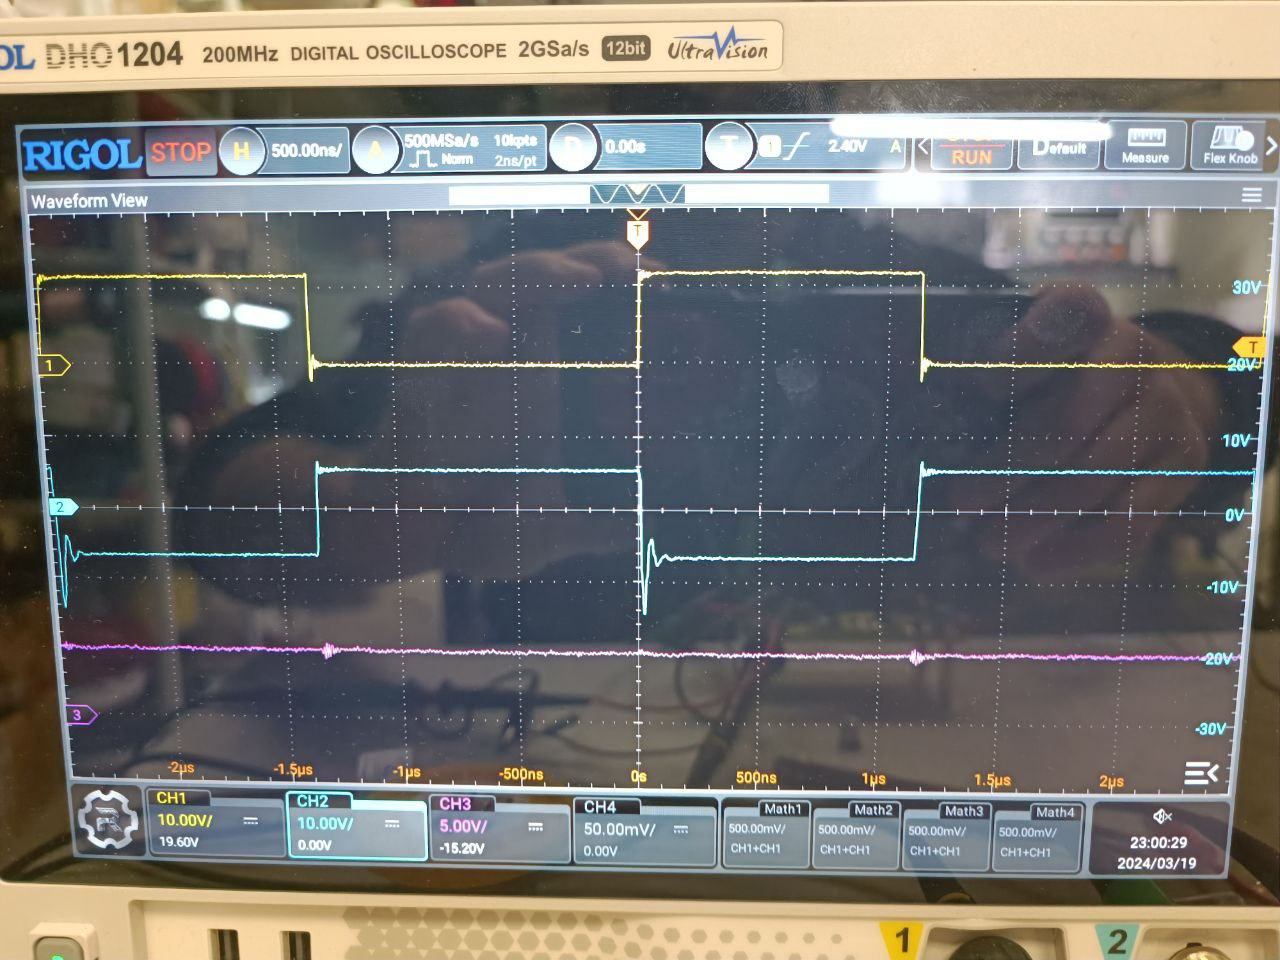
\includegraphics[scale = 0.4]{ris331.jpeg}
    \caption{Осциллограммы при входном напряжении 12 В}
    \label{ris:331}
\end{figure}

Здесь и далее желтый сигнал -- на выводе SW, развертка по напряжению 10 В/деление. Голубой сигнал -- падение 
напряжения на диоде (VD7, рисунка \ref{ris:321}), равертка по напряжению 10 В/деление. Фиолетовый сигнал -- 
контроль напряжения на изолированном выходе (контрольная точка CP5, рисунка \ref{ris:321}), развертка
по напряжению 5 В, нагрузка - 10 Ом. 

Осцилограммы при входном напряжении 18 В представлены на рисунке \ref{ris:332}:

\begin{figure}[H]
    \centering
    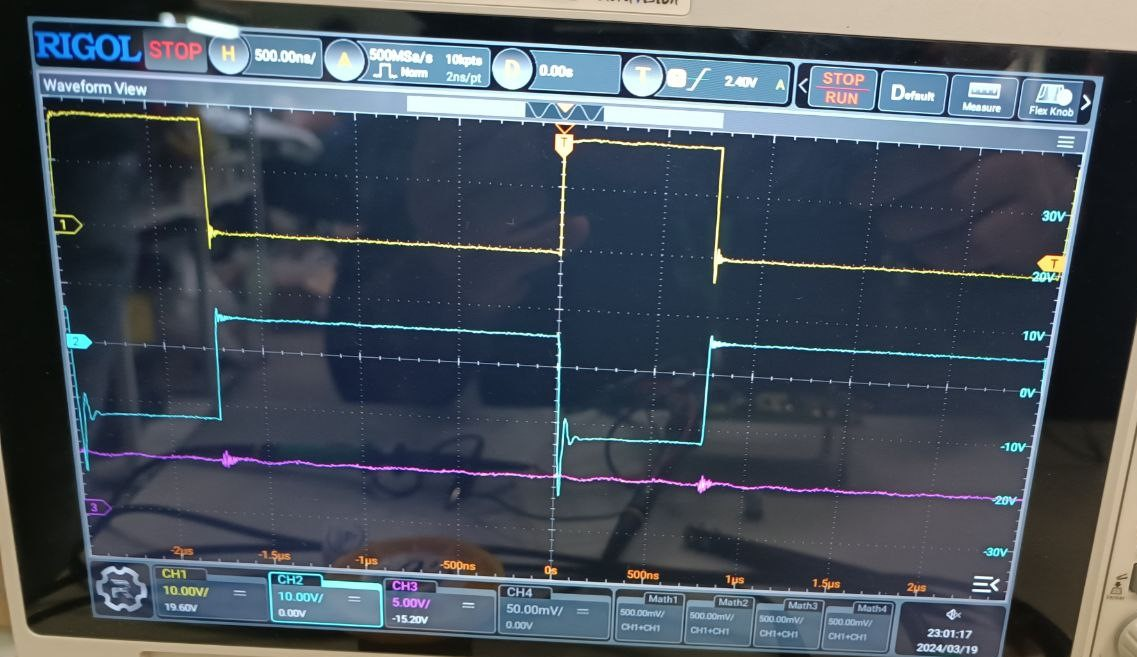
\includegraphics[scale = 0.6]{ris332.jpeg}
    \caption{Осциллограммы при входном напряжении 18 В}
    \label{ris:332}
\end{figure}

Осцилограммы при входном напряжении 24 В представлены на рисунке \ref{ris:333}:

\begin{figure}[H]
    \centering
    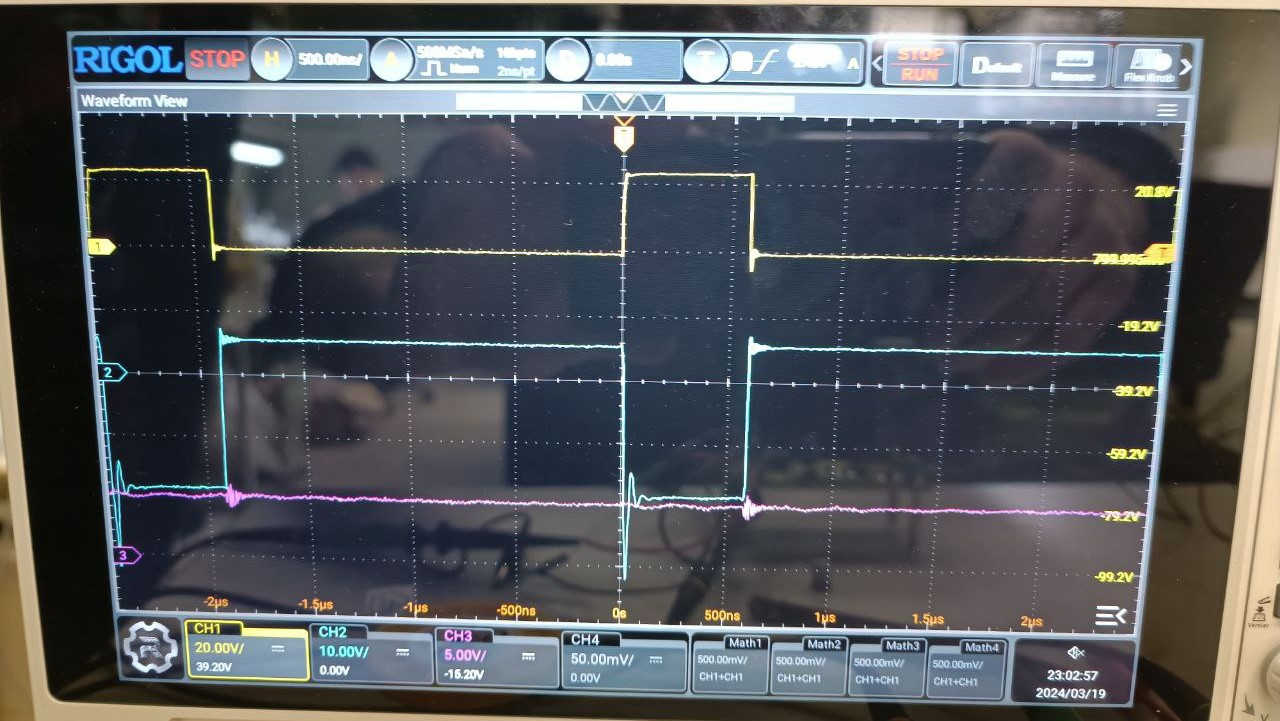
\includegraphics[scale = 0.5]{ris333.jpeg}
    \caption{Осциллограммы при входном напряжении 24 В}
    \label{ris:333}
\end{figure}

Здесь поменялась развертка желтого сигнала на 20 В/деление. 

Осцилограммы при входном напряжении 36 В представлены на рисунке \ref{ris:334}:

\begin{figure}[H]
    \centering
    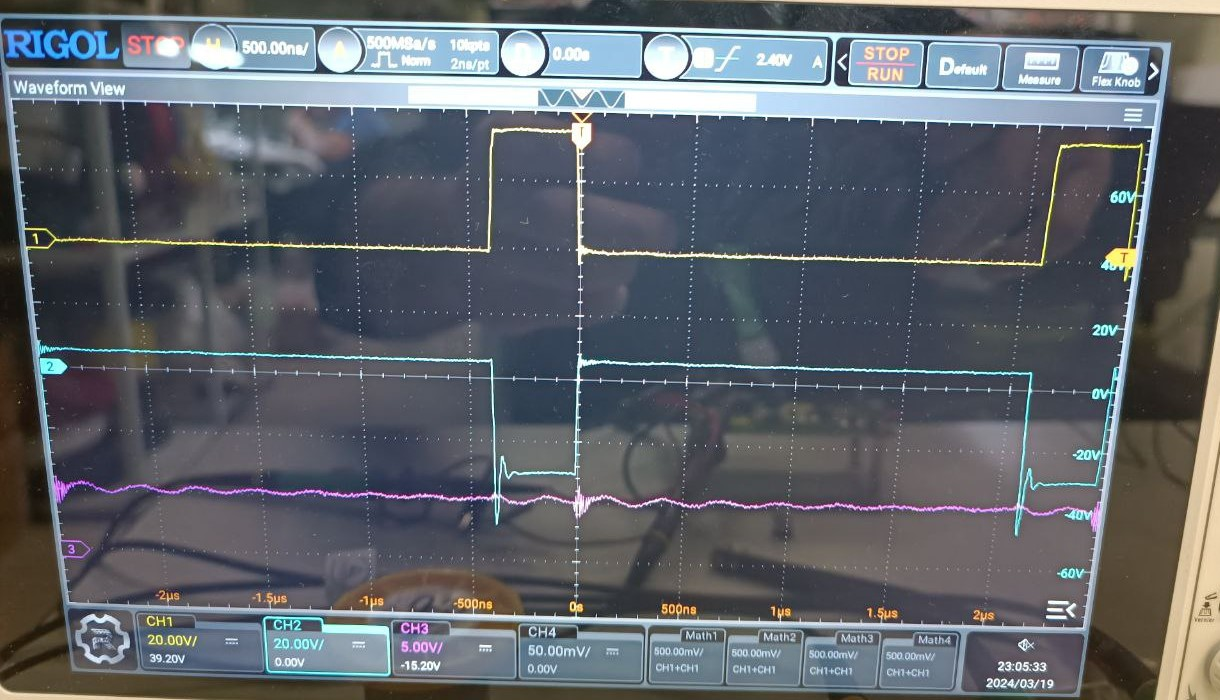
\includegraphics[scale = 0.55]{ris334.jpeg}
    \caption{Осциллограммы при входном напряжении 36 В}
    \label{ris:334}
\end{figure}

Здесь поменялась развертка голубого сигнала на 20 В/деление. 

Осцилограммы при входном напряжении 48 В представлены на рисунке \ref{ris:335}:

\begin{figure}[H]
    \centering
    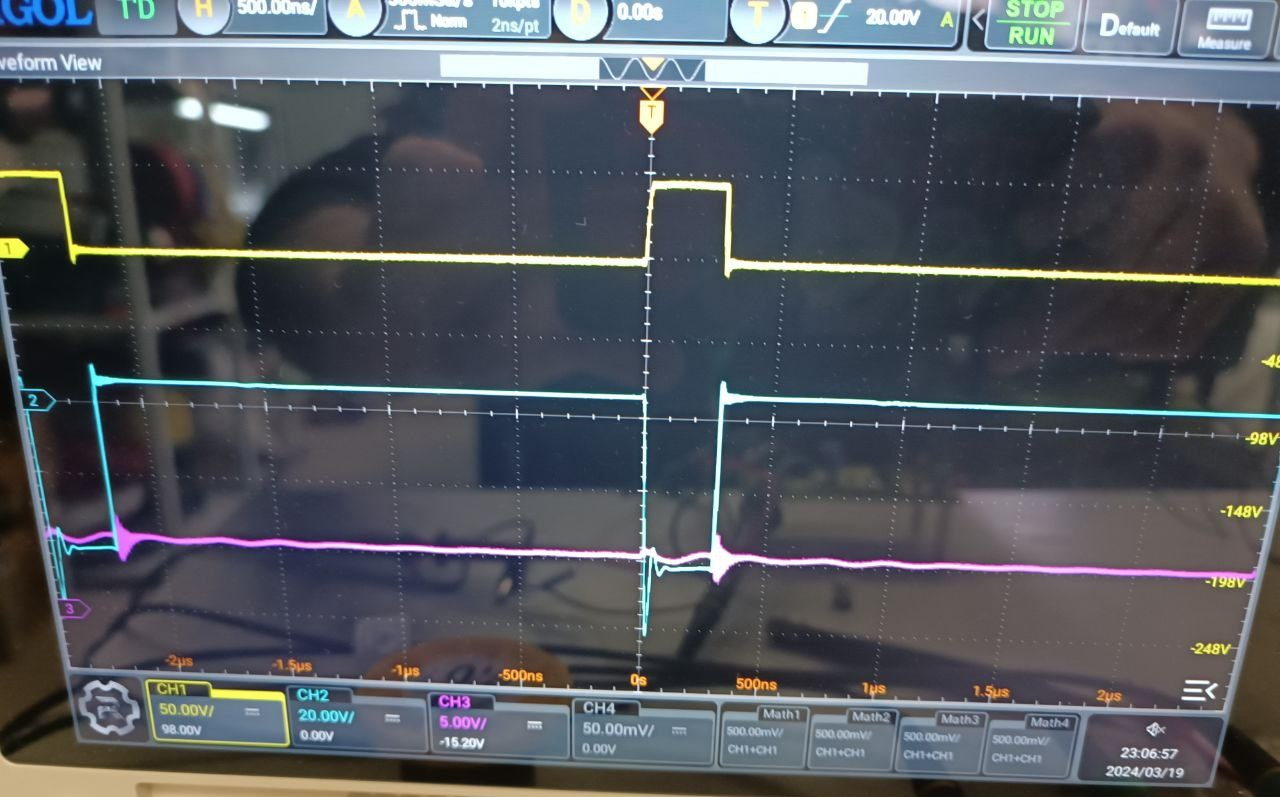
\includegraphics[scale = 0.5]{ris335.jpeg}
    \caption{Осциллограммы при входном напряжении 48 В}
    \label{ris:335}
\end{figure}

Здесь поменялась развертка желтого сигнала на 50 В/деление. Уменьшим развертку по веремени до 100 нс/деление
и рассмотрим осциллограммы на рисунке \ref{ris:336}


\begin{figure}[H]
    \centering
    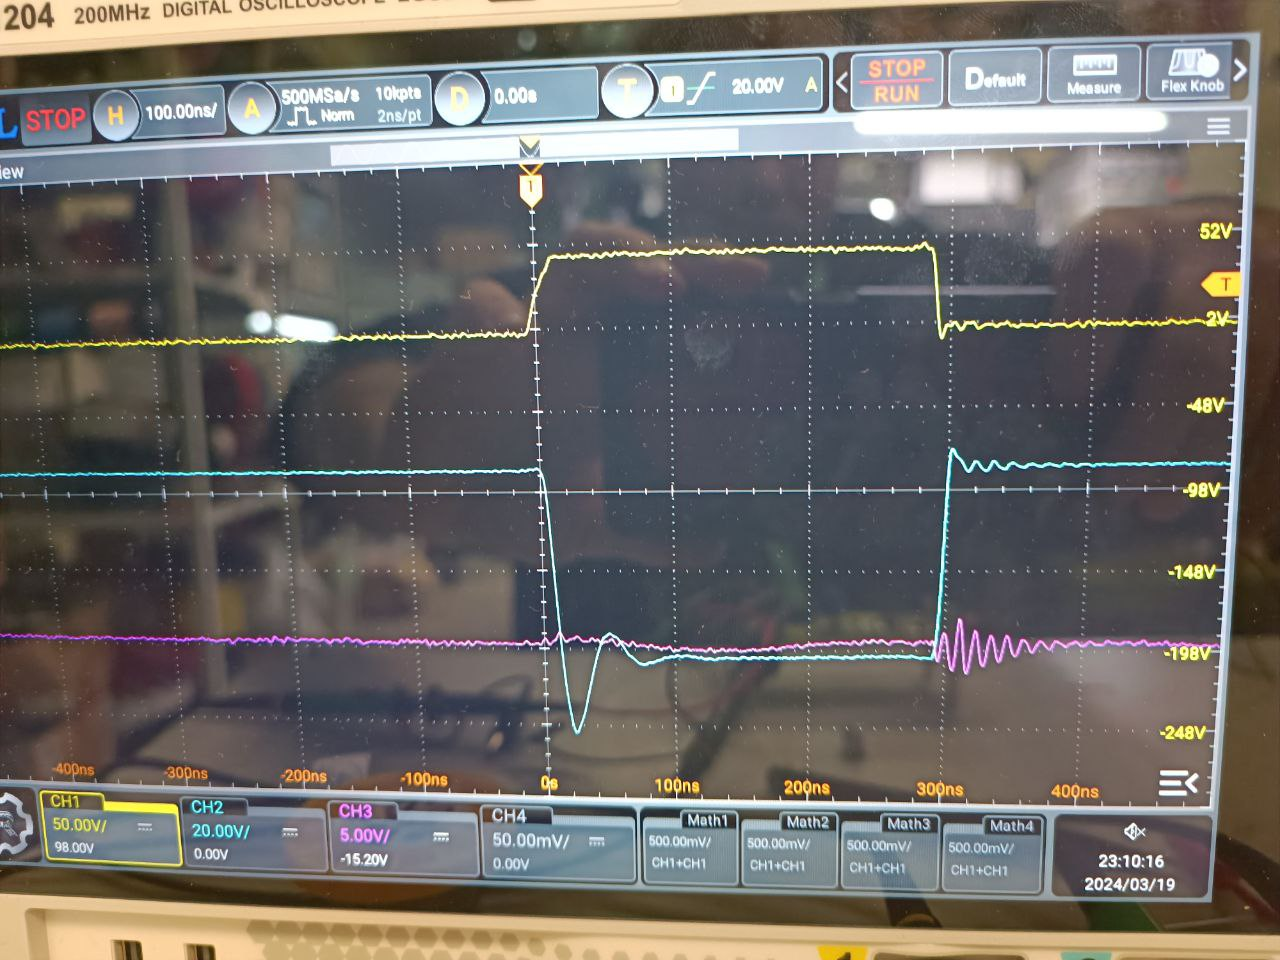
\includegraphics[scale = 0.4]{ris336.jpeg}
    \caption{Увеличенные осциллограммы при входном напряжении 48 В}
    \label{ris:336}
\end{figure}

На диоде (голубой сигнал), отчетливо видны выбросы индуктивности при переключении внутреннего транзистора. 
Ампилтуда этих выбросов составляет -62 В при включении транзистора, и примерно 4 В при выключении.
Амплитуда отрицательных выбросов говорит нам о том, что следует заменить диод на тот, обратное напряжение которого
составляет хотя бы 100 В, а не 60, как сейчас. Основные искажения на изолированое питание вносят выбросы при 
выключении транзистора, апмлитуда которых составляет примерно 1,5 В (размах 3 В), а частота 66,67 МГц. 
Расположенный дальше по схеме стабилизатор должен спокойно выдержать такие амлитуды выбросов, так же при
проектировании подсистемы питания мы закладывали возможность повышения выходного напряжения изолированного 
выхода до 6,5 В, что вписывается в расчетные данные. В случае неправильной работы LDO, можно будет попробовать
подавить высокочастотные выбросы добавлением входного конденсатора по входу стабилизатора 3,3 В.

Далее проаннализируем работу PoE-преобразователя. Для понимания правильности его работы достаточно посмотреть
на осцилограмму на рисунке \ref{ris:337}:

\begin{figure}[H]
    \centering
    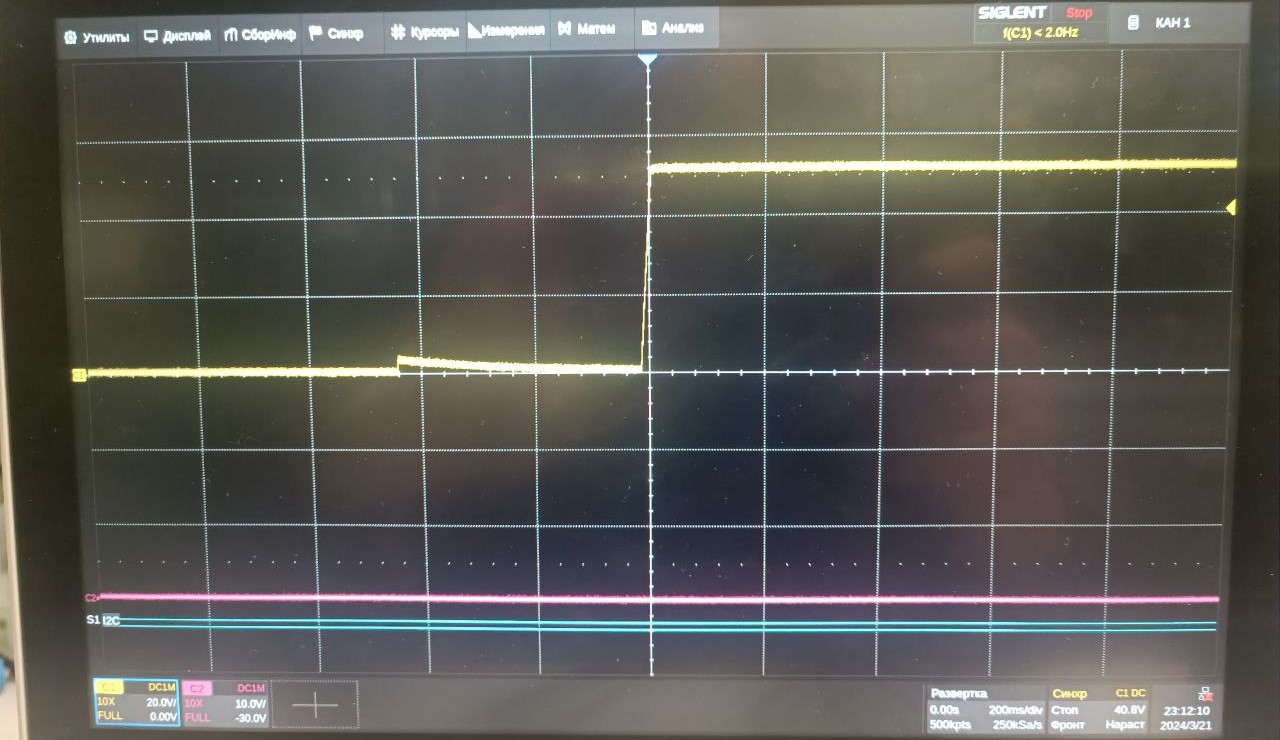
\includegraphics[scale = 0.45]{ris337.jpeg}
    \caption{Осцилограммы при старте работы PoE-контроллера}
    \label{ris:337}
\end{figure}

где, желтая осцилограмма -- вывод VDD, развертка по напряжению 20 В/деление, а по времени 200 мс/деление. 
В качестве нагрузки стоит LMR36520 нагруженный на 10 Ом.
Здесь можно заметить ярко выраженную стадию detection, которая длится 
примерно 100 мс, что соответсвует документации на TPS2376. Этап классификации утройства проходит линейно и 
дальше контроллер выходит на напряжение питания равное прмиерно 60 В. 

За исключением выбросов на диоде VD7, схема работает как планировалось, расчеты соответсвтуют действительности.
 % описание принципа работы системы питания
\chapter{Описание принципа работы подсистемы измерения энергопотребления}
\section{Обоснование выбора компонентов измерительной части}
\subsection{Операционный усилитель}
\hspace{1cm} 

Вопрос какой операционный усилитель (далее ОУ) использовать в качестве дифференциального усилителя -- самый 
критичный для подсистемы измерения энергопотребления. Прежде всего стоит определиться с требованиями к 
самым важным параметрам ОУ. 
Одной из важных характеристик операционного усилителя (ОУ) является напряжение смещения $V_{os}$ — или, 
говоря проще, напряжение ошибки на его входах. Любой неидеальный ОУ при отсутствии входного сигнала выдаёт 
выходной так, как будто бы на самом деле вход-ной сигнал равен Vos.

Напряжение смещения обычно составляет от единиц микровольт до единиц милливольт — и, соответственно, 
доставляет серьёзные неудобства при работе с низковольтными источни-ками: термопарами, шунтами и так далее.
Особенно — если оно отрицательное, а схема однополярная: тогда на выходе ОУ будет просто 0, пока 
напряжение входного сигнала не превысит Vos, и никакой калибровкой это устранить невозможно \cite{Chopper:OU} 
\cite{MT-037:Tutorial}. 

При измерении микро- и милиамперных диапазонов высокое напряжение смещение мо-жет стать проблемой.
Для этого следует изучить реальную зависимость напряжения смещения от Vcm и сравнить ее с той, 
которую приводят в datasheet, как, например, на рисунке \ref{ris:411} \cite{OPAx376:datasheet}.
\begin{figure}[H]
\centering
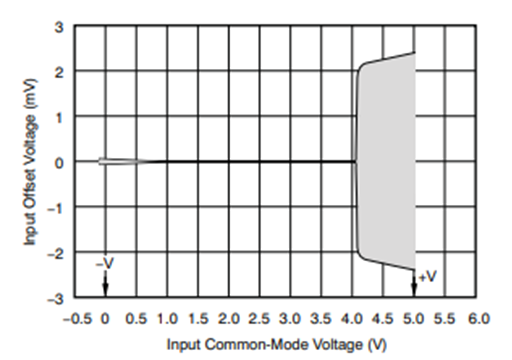
\includegraphics[scale = 1]{ris411.png}
\caption{Зависимость напряжения смещения от $V_{cm}$}
\label{ris:411}
\end{figure}

Так же стоит посмотреть на напряжение смещения в зависимости от ОУ в партии, 
на рисунке \ref{ris:412} представлен график для OPA2376 \cite{OPAx376:datasheet}

\begin{figure}[H]
\centering
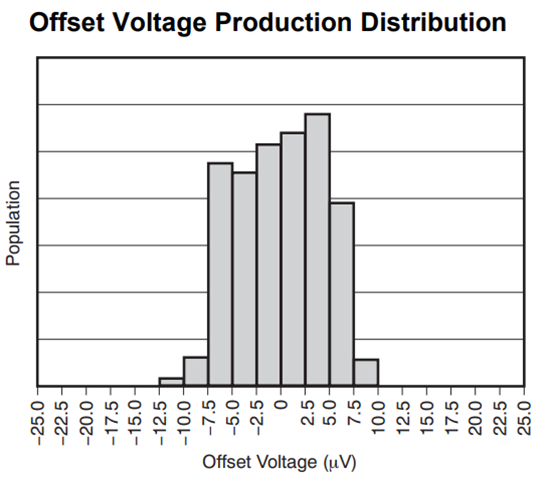
\includegraphics[scale = 1]{ris412.png}
\caption{Показатель напряжения смещения в рамках одной партии}
\label{ris:412}
\end{figure}

Также стоит упомянуть про то, что при использовании автоматического переключения шунтов 
чоппер-стабилизированные ОУ малопригодны из-за долгого времени восстановления, так как из-за частоты работы
АЦП порядка сотен кГц, время переключения свыше 1 мкс нам не подходит \cite{Chopper:OU}.

Исходя из вышесказанного, можно изучить следующие ОУ:

\begin{itemize}
    \item OPA2376 от Texas Instruments -- прецизионный rail-to-rail, выполненный по технологии etrim
    \item OPA2376 от Fulihao -- прецизионный rail-to-rail, выполненный по технологии etrim
    \item AD8606 от Analoc Device -- прецизионный rail-to-rail, выполненный по технологии etrim
    \item TP2312 -- прецизионный малошумящий rail-to-rail
    \item RS8552 -- чоппер-стабилизированный
    \item RS8562 -- чоппер-стабилизированный
\end{itemize}

На выбор ОУ влияла так же возможность быстро и без проблем приобрести на территории РФ. 

На рисунке \ref{ris:413} представлена схема измерения напряжения смещения.

\begin{figure}[H]
    \centering
    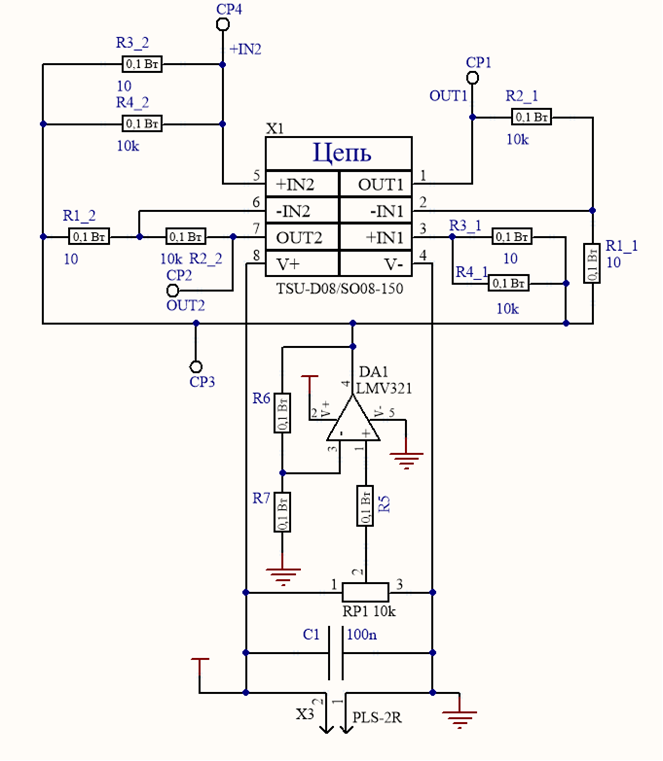
\includegraphics[scale = 0.9]{ris413.png}
    \caption{Схема измерительной установки}
    \label{ris:413}
    \end{figure}

Здесь Х1 -- контактирующее устройство, предназначенное для быстрой смены операци-онного усилителя в 
корпусе SOIC-8 -- самого распространённого типа корпуса для ОУ. Испытуемый ОУ включён по схеме неинвертирующего 
усилителя с коэффициентом усиления 1000, который обеспечивается резисторами R2\_1 и R1\_1 для первого ОУ и
резисторами R2\_2 и R1\_2 для второго ОУ в корпусе. DA1 с обвязкой к нему выполняет роль буферного ОУ для 
обеспечения лучшего импеданса и большей нагрузочной способности при низком токе через делитель R3 и R4.

Данная схема позволит преобразовать микровольтное напряжение смещение в миливольты, что достаточно для 
измерения обычным вольтметром. Подстроечным резистором RP1 регулируется input common-mode voltage, как 
на рисунке \ref{ris:411}. Напряжение питание схемы 5 В.

% Table generated by Excel2LaTeX from sheet 'Vcm' and from my teardrops
\begin{table}[H]
    \begin{adjustwidth}{-1em}{}
    \centering
    \caption{Результаты измерений напряжения смещения у разных ОУ}
      \begin{tabular}{|c|c|c|c|c|c|c|c|c|c|c|c|}
      \hline
      \multicolumn{1}{|c|}{\multirow{3}[6]{2cm}{\textbf{Тип ОУ}}} & \multicolumn{1}{c|}{\multirow{3}[6]{1.4cm}{\textbf{Номер экземпляра}}} & \multicolumn{1}{c|}{\multirow{3}[6]{1.8cm}{\textbf{Номер ОУ в корпусе}}} & \multicolumn{9}{|c|}{\textbf{Напряжение смещения, мВ}} \bigstrut\\
  \cline{4-12}          &       &       & \multicolumn{9}{|c|}{\textbf{При Vcm, В}} \bigstrut\\
  \cline{4-12}          &       &       & \textbf{0,5} & \textbf{1} & \textbf{1,5} & \textbf{2} & \textbf{2,5} & \textbf{3} & \textbf{3,5} & \textbf{4} & \textbf{4,5} \bigstrut\\
      \hline
      \multicolumn{1}{|c|}{\multirow{10}[20]{*}{OPA2376 }} & \multirow{2}[4]{*}{1} & 1     & 13,4  & 7,9   & 2,4   & -2,4  & -8,1  & -11,8 & -15,3 & -12,8 & 483 \bigstrut\\
  \cline{3-12}          &       & 2     & 4,2   & 6     & 4,3   & 2,3   & -1    & -3,5  & -6    & -9,7  & -1813 \bigstrut\\
  \cline{2-12}          & \multirow{2}[4]{*}{2} & 1     & 28,5  & 18,7  & 9,3   & 0,3   & -8    & -15,2 & -22,7 & -58,5 & -388 \bigstrut\\
  \cline{3-12}          &       & 2     & -5,5  & -7,5  & -8,5  & -6,8  & -6,1  & -3,9  & -1,9  & -8,9  & -680 \bigstrut\\
  \cline{2-12}          & \multirow{2}[4]{*}{3} & 1     & 26,7  & 20,3  & 14,2  & 9,1   & 3,6   & -0,2  & -4,4  & -16,6 & -2230 \bigstrut\\
  \cline{3-12}          &       & 2     & -55,7 & -33,4 & -21,7 & -12,3 & -7,3  & -1,5  & 2,9   & -10,9 & -4500 \bigstrut\\
  \cline{2-12}   TI     & \multirow{2}[4]{*}{4} & 1     & -18,2 & -10,8 & -6,3  & -2,5  & 0,1   & 2,5   & 4,6   & 14,5  & -1532 \bigstrut\\
  \cline{3-12}          &       & 2     & 7,2   & 5,5   & -0,1  & -4,8  & -9,2  & -13,4 & -17,2 & -23,3 & -1517 \bigstrut\\
  \cline{2-12}          & \multirow{2}[4]{*}{5} & 1     & -18,8 & -10,4 & -4,5  & 0,2   & 3,2   & 6,3   & 8,6   & 22    & 395 \bigstrut\\
  \cline{3-12}          &       & 2     & -70,4 & -43,6 & -24,7 & -11,2 & -1,6  & 7,5   & 14,4  & 30    & 624 \bigstrut\\
      \hline
      \multicolumn{1}{|c|}{\multirow{6}[12]{*}{OPA2376}} & \multirow{2}[4]{*}{1} & 1     & -6,3  & -6,5  & -8,4  & -8,2  & -7,35 & -7,9  & -10   & -5,9  & -4,6 \bigstrut\\
  \cline{3-12}          &       & 2     & -2,8  & -2,9  & -4,5  & -4,3  & -3,1  & -3,3  & -4,7  & -2,7  & -1,7 \bigstrut\\
  \cline{2-12}          & \multirow{2}[4]{*}{2} & 1     & -6,8  & -6,8  & -9    & -9    & -8,01 & -8,9  & -10,4 & -11,8 & -10,1 \bigstrut\\
  \cline{3-12}          &       & 2     & 1,3   & 1     & -0,6  & -0,5  & 0,2   & 1,2   & -0,1  & 2     & 3,4 \bigstrut\\
  \cline{2-12} Fulihao   & \multirow{2}[4]{*}{3} & 1     & -4,6  & -4,4  & -6,4  & -6,8  & -6,4  & -6,5  & -8,5  & -7,7  & -6,2 \bigstrut\\
  \cline{3-12}          &       & 2     & -1,4  & -1,2  & -2,3  & -2,1  & -0,8  & -0,6  & -2,3  & -1,5  & 0,2 \bigstrut\\
      \hline
      \multicolumn{1}{|c|}{\multirow{10}[20]{*}{AD8606}} & \multirow{2}[4]{*}{1} & 1     & 40,1  & 36,3  & 33,7  & 33,5  & 31,3  & 30,6  & 3,5   & 6,2   & 19,8 \bigstrut\\
  \cline{3-12}          &       & 2     & 11,4  & 32,8  & 49,3  & 59,67 & 72    & 80,5  & 19,2  & -10,4 & -13,6 \bigstrut\\
  \cline{2-12}          & \multirow{2}[4]{*}{2} & 1     & 21,4  & 27,2  & 31,3  & 34,5  & 36,1  & 38,3  & 87,5  & 73,8  & 93,6 \bigstrut\\
  \cline{3-12}          &       & 2     & 12,8  & 4,6   & 0,6   & -0,3  & -2,2  & -2,1  & -94,4 & -39,9 & -46,5 \bigstrut\\
  \cline{2-12}          & \multirow{2}[4]{*}{3} & 1     & 17,8  & 34,3  & 47,5  & 59,2  & 71,8  & 84,9  & 29,7  & 29,5  & 23,6 \bigstrut\\
  \cline{3-12}          &       & 2     & -16,3 & -3,3  & 6,6   & 13,9  & 1,3   & 27,9  & 48,8  & 9,3   & 15,6 \bigstrut\\
  \cline{2-12}          & \multirow{2}[4]{*}{4} & 1     & 74,7  & 63,5  & 51,1  & 40,5  & 31,9  & 24,1  & 40,9  & 61,6  & 73,7 \bigstrut\\
  \cline{3-12}          &       & 2     & 15,3  & -6,9  & -25,1 & -38,5 & -51,4 & -64,2 & -53,8 & -17,5 & -29,4 \bigstrut\\
  \cline{2-12}          & \multirow{2}[4]{*}{5} & 1     & 59,5  & 51,8  & 41,9  & 35,3  & 24,8  & 18,3  & 10,4  & 0,9   & 11,8 \bigstrut\\
  \cline{3-12}          &       & 2     & 14,9  & 22,5  & 32,1  & 37,4  & 44,2  & 48,6  & 35,2  & 35,7  & 40,4 \bigstrut\\
      \hline
      \multicolumn{1}{|c|}{\multirow{10}[20]{*}{TP2312}} & \multirow{2}[4]{*}{1} & 1     & 17,4  & 18,2  & 18,8  & 20,6  & 23,3  & 26,5  & 28,9  & 165,9 & -1072 \bigstrut\\
  \cline{3-12}          &       & 2     & 30,4  & 38,6  & 43,6  & 47,9  & 49,7  & 50,6  & 51,2  & -41,7 & -1550 \bigstrut\\
  \cline{2-12}          & \multirow{2}[4]{*}{2} & 1     & -12,4 & -10,2 & -7    & -2,6  & 3,2   & 7     & 12,9  & -391  & -3330 \bigstrut\\
  \cline{3-12}          &       & 2     & 8,3   & 14,9  & 19,3  & 22,4  & 26,9  & 30,8  & 34,2  & 24,3  & -1183 \bigstrut\\
  \cline{2-12}          & \multirow{2}[4]{*}{3} & 1     & 12,8  & 6,6   & 2,3   & -4,2  & -10,9 & -16,9 & 46,3  & 34,9  & -403 \bigstrut\\
  \cline{3-12}          &       & 2     & 16,2  & 15,4  & 17,1  & 19,4  & 23    & 27,5  & 51,2  & 330   & -1491 \bigstrut\\
  \cline{2-12}          & \multirow{2}[4]{*}{4} & 1     & -24,1 & -16,9 & -11   & -4,3  & 0,5   & 4,1   & 8,4   & 269   & -2530 \bigstrut\\
  \cline{3-12}          &       & 2     & 3,7   & 3,9   & 4,5   & 6,8   & 9,1   & 12,9  & 16,7  & 468   & -1950 \bigstrut\\
  \cline{2-12}          & \multirow{2}[4]{*}{5} & 1     & 3,6   & -13,8 & -23,8 & -31,8 & -38,5 & -43,8 & -47,3 & -123,2 & -2660 \bigstrut\\
  \cline{3-12}          &       & 2     & 28,2  & 23    & 18,5  & 14    & 8,8   & 5,3   & 1,3   & 934   & -171 \bigstrut\\
      \hline
      \end{tabular}%
    \label{tab:Vcm1}%
    \end{adjustwidth}
  \end{table}



  \begin{table}[H]
    %\begin{adjustwidth}{-2em}{}
    \centering
    \caption{Результаты измерений напряжения смещения у разных ОУ}
      \begin{tabular}{|c|c|c|c|c|c|c|c|c|c|c|c|}
      \hline
      \multicolumn{1}{|c|}{\multirow{3}[6]{2cm}{\textbf{Тип ОУ}}} & \multicolumn{1}{c|}{\multirow{3}[6]{1.4cm}{\textbf{Номер экземпляра}}} & \multicolumn{1}{c|}{\multirow{3}[6]{1.8cm}{\textbf{Номер ОУ в корпусе}}} & \multicolumn{9}{|c|}{\textbf{Напряжение смещения, мВ}} \bigstrut\\
  \cline{4-12}          &       &       & \multicolumn{9}{|c|}{\textbf{При Vcm, В}} \bigstrut\\
  \cline{4-12}          &       &       & \textbf{0,5} & \textbf{1} & \textbf{1,5} & \textbf{2} & \textbf{2,5} & \textbf{3} & \textbf{3,5} & \textbf{4} & \textbf{4,5} \bigstrut\\
      \hline
      \multicolumn{1}{|c|}{\multirow{10}[20]{*}{RS8552}} & \multirow{2}[4]{*}{1} & 1     & -0,1  & -0,4  & -0,5  & 0,3   & -0,6  & -0,4  & 0,9   & -0,8  & -0,5 \bigstrut\\
  \cline{3-12}          &       & 2     & -1,3  & -0,5  & -0,4  & -0,1  & -0,5  & 0,6   & -0,2  & -0,2  & -0,9 \bigstrut\\
  \cline{2-12}          & \multirow{2}[4]{*}{2} & 1     & -0,3  & -0,4  & -0,1  & -0,4  & -0,2  & -0,3  & -0,2  & -0,6  & -5 \bigstrut\\
  \cline{3-12}          &       & 2     & -0,4  & -0,2  & 0     & -0,1  & -0,8  & -0,5  & -0,3  & -0,5  & -0,5 \bigstrut\\
  \cline{2-12}          & \multirow{2}[4]{*}{3} & 1     & -0,5  & 0,5   & 0,2   & -0,6  & -0,2  & -0,9  & -0,7  & -0,3  & -0,4 \bigstrut\\
  \cline{3-12}          &       & 2     & -0,3  & -0,6  & -0,3  & -0,2  & -0,3  & -0,2  & -0,8  & -0,4  & -0,5 \bigstrut\\
  \cline{2-12}          & \multirow{2}[4]{*}{4} & 1     & 0,8   & 1,1   & 1,4   & 1     & 0,8   & -0,7  & -0,1  & -0,6  & -0,3 \bigstrut\\
  \cline{3-12}          &       & 2     & -0,6  & -0,4  & -0,6  & -0,2  & -0,4  & -0,3  & -0,1  & -0,7  & -0,9 \bigstrut\\
  \cline{2-12}          & \multirow{2}[4]{*}{5} & 1     & -0,4  & 0,1   & -0,4  & -0,1  & -0,2  & -0,2  & -0,3  & -0,5  & -0,4 \bigstrut\\
  \cline{3-12}          &       & 2     & -0,3  & -0,3  & -0,2  & -0,5  & -0,2  & -0,1  & -0,6  & -0,5  & -0,6 \bigstrut\\
      \hline
      \multicolumn{1}{|c|}{\multirow{10}[20]{*}{RS8562}} & \multirow{2}[4]{*}{1} & 1     & -1,3  & -0,6  & -0,4  & -0,3  & -0,1  & -0,9  & -0,4  & -0,6  & -0,1 \bigstrut\\
  \cline{3-12}          &       & 2     & -1,3  & -0,4  & -0,9  & -0,5  & -0,8  & -0,3  & -0,4  & -0,8  & -0,7 \bigstrut\\
  \cline{2-12}          & \multirow{2}[4]{*}{2} & 1     & 0,1   & 0,5   & 0,1   & -0,6  & 0,5   & -0,2  & -0,2  & -0,2  & 0,3 \bigstrut\\
  \cline{3-12}          &       & 2     & -1,2  & -0,9  & -1    & -0,5  & -0,2  & -0,9  & -0,2  & -0,5  & -0,8 \bigstrut\\
  \cline{2-12}          & \multirow{2}[4]{*}{3} & 1     & 0     & 0,3   & 0,2   & -0,2  & 0,6   & -0,8  & -0,7  & -0,6  & 0,4 \bigstrut\\
  \cline{3-12}          &       & 2     & -0,8  & -0,1  & -1,2  & -0,1  & -0,1  & -0,4  & -0,6  & -0,6  & -0,9 \bigstrut\\
  \cline{2-12}          & \multirow{2}[4]{*}{4} & 1     & 0,2   & 0,6   & -0,3  & -0,7  & -0,2  & -0,9  & -0,7  & -0,2  & -0,1 \bigstrut\\
  \cline{3-12}          &       & 2     & -1,8  & -1,5  & -2,1  & -0,6  & -0,6  & -0,1  & -0,7  & -0,4  & -0,8 \bigstrut\\
  \cline{2-12}          & \multirow{2}[4]{*}{5} & 1     & -0,1  & 0,2   & 0,4   & -0,9  & 0,3   & -0,6  & -0,8  & 0,1   & -0,6 \bigstrut\\
  \cline{3-12}          &       & 2     & -1,6  & -1    & -0,6  & -0,4  & -0,5  & -0,9  & -0,1  & -0,9  & -0,7 \bigstrut\\
      \hline
      \end{tabular}%
    \label{tab:Vcm2}%
    %\end{adjustwidth}
  \end{table}
%\end{landscape}
В данной таблице результаты измерения после усиления напряжения смещения в 1000 раз. Из результатов измерений
можно сказать, что заявленное производителями напряжение смещения соответствует измеренным


\section{Расчет элементов схемы}
\hspace{1cm} 

\section{Результаты тестирования}
\hspace{1cm}  % описание принципа работы измерительной части
\begin{thebibliography}{00}

\addcontentsline{toc}{chapter}{Список используемой литературы}

\bibitem{Lakamera:embed} Лакамера, Д.
\emph{Архитектура встраиваемых систем} /Д. Лакамера // ДМК Пресс --
Москва -- 2023. -- 332 с.

\bibitem{STM32:datasheet} Connectivity line, ARM®-based 32-bit MCU with 64/256 KB Flash,
 USB OTG, Ethernet, 10 timers, 2 CANs, 2 ADCs, 14 communication interfaces -- datasheet/
  [Электронный ресурс]
 /STMicroelectronics// -- Март, 2017 -- 
 URL:https://www.st.com/resource/en/datasheet/stm32f107vc.pdf --
 (Дата обращения: 15.05.2024)

\bibitem{TPS2376:datasheet} IEEE 802.3af PoE POWERED DEVICE CONTROLLERS -- datasheet/
  [Электронный ресурс] /Texas Instrument// -- Апрель, 2008 
  -- URL:https://www.ti.com/lit/ds/symlink/tps2376.pdf?ts=1715733862395 --
  (Дата обращения: 15.05.2024)

\bibitem{DP83848:datasheet} DP83848-EP PHYTER™ Military Temperature Single Port
   10/100 Mbps Ethernet
  Physical Layer Transceiver -- datasheet/
  [Электронный ресурс] /Texas Instrument// -- Июнь, 2019 
  -- URL:https://www.ti.com/lit/ds/symlink/dp83848-ep.pdf --
  (Дата обращения: 15.05.2024)

\bibitem{HorHill:ArtOfScheme} Хоровиц, П.
\emph{Искусство схемотехники издание седьмое} /П. Хоровиц, У. Хилл // <<Бином>> --
Москва -- 2003. -- 704 с.

\bibitem{PowerElectronic:FlyBack} Обратноходовой преобразователь /
  [Электронный ресурс] /Алфавит силовой электроники// 
   URL:https://www.power-electronics.info/flyback.html --
  (Дата обращения: 15.05.2024)

\bibitem{GooglePatent:1} M. G. Liberty, “Auto ranging ammeter with accurate measurement 
during range changes. -- URL:
https://patents.google.com/patent/US11774469B2 (Дата обращения: 31.03.2024).

\bibitem{SN74LVC2T45:datasheet} 2-Bit Dual Supply Transceiver with Configurable 
Voltage-Level Shifting and 3-State Outputs
 -- datasheet/
  [Электронный ресурс] /Texas Instrument// -- Октябрь, 2022 -- 
  URL: https://www.ti.com/product/SN74LVC2T45
   --(Дата обращения: 15.05.2024)

\end{thebibliography}
 % ссылки на литературу
\end{document}